\documentclass[1p]{elsarticle_modified}
%\bibliographystyle{elsarticle-num}

%\usepackage[colorlinks]{hyperref}
%\usepackage{abbrmath_seonhwa} %\Abb, \Ascr, \Acal ,\Abf, \Afrak
\usepackage{amsfonts}
\usepackage{amssymb}
\usepackage{amsmath}
\usepackage{amsthm}
\usepackage{scalefnt}
\usepackage{amsbsy}
\usepackage{kotex}
\usepackage{caption}
\usepackage{subfig}
\usepackage{color}
\usepackage{graphicx}
\usepackage{xcolor} %% white, black, red, green, blue, cyan, magenta, yellow
\usepackage{float}
\usepackage{setspace}
\usepackage{hyperref}

\usepackage{tikz}
\usetikzlibrary{arrows}

\usepackage{multirow}
\usepackage{array} % fixed length table
\usepackage{hhline}

%%%%%%%%%%%%%%%%%%%%%
\makeatletter
\renewcommand*\env@matrix[1][\arraystretch]{%
	\edef\arraystretch{#1}%
	\hskip -\arraycolsep
	\let\@ifnextchar\new@ifnextchar
	\array{*\c@MaxMatrixCols c}}
\makeatother %https://tex.stackexchange.com/questions/14071/how-can-i-increase-the-line-spacing-in-a-matrix
%%%%%%%%%%%%%%%

\usepackage[normalem]{ulem}

\newcommand{\msout}[1]{\ifmmode\text{\sout{\ensuremath{#1}}}\else\sout{#1}\fi}
%SOURCE: \msout is \stkout macro in https://tex.stackexchange.com/questions/20609/strikeout-in-math-mode

\newcommand{\cancel}[1]{
	\ifmmode
	{\color{red}\msout{#1}}
	\else
	{\color{red}\sout{#1}}
	\fi
}

\newcommand{\add}[1]{
	{\color{blue}\uwave{#1}}
}

\newcommand{\replace}[2]{
	\ifmmode
	{\color{red}\msout{#1}}{\color{blue}\uwave{#2}}
	\else
	{\color{red}\sout{#1}}{\color{blue}\uwave{#2}}
	\fi
}

\newcommand{\Sol}{\mathcal{S}} %segment
\newcommand{\D}{D} %diagram
\newcommand{\A}{\mathcal{A}} %arc


%%%%%%%%%%%%%%%%%%%%%%%%%%%%%5 test

\def\sl{\operatorname{\textup{SL}}(2,\Cbb)}
\def\psl{\operatorname{\textup{PSL}}(2,\Cbb)}
\def\quan{\mkern 1mu \triangleright \mkern 1mu}

\theoremstyle{definition}
\newtheorem{thm}{Theorem}[section]
\newtheorem{prop}[thm]{Proposition}
\newtheorem{lem}[thm]{Lemma}
\newtheorem{ques}[thm]{Question}
\newtheorem{cor}[thm]{Corollary}
\newtheorem{defn}[thm]{Definition}
\newtheorem{exam}[thm]{Example}
\newtheorem{rmk}[thm]{Remark}
\newtheorem{alg}[thm]{Algorithm}

\newcommand{\I}{\sqrt{-1}}
\begin{document}

%\begin{frontmatter}
%
%\title{Boundary parabolic representations of knots up to 8 crossings}
%
%%% Group authors per affiliation:
%\author{Yunhi Cho} 
%\address{Department of Mathematics, University of Seoul, Seoul, Korea}
%\ead{yhcho@uos.ac.kr}
%
%
%\author{Seonhwa Kim} %\fnref{s_kim}}
%\address{Center for Geometry and Physics, Institute for Basic Science, Pohang, 37673, Korea}
%\ead{ryeona17@ibs.re.kr}
%
%\author{Hyuk Kim}
%\address{Department of Mathematical Sciences, Seoul National University, Seoul 08826, Korea}
%\ead{hyukkim@snu.ac.kr}
%
%\author{Seokbeom Yoon}
%\address{Department of Mathematical Sciences, Seoul National University, Seoul, 08826,  Korea}
%\ead{sbyoon15@snu.ac.kr}
%
%\begin{abstract}
%We find all boundary parabolic representation of knots up to 8 crossings.
%
%\end{abstract}
%\begin{keyword}
%    \MSC[2010] 57M25 
%\end{keyword}
%
%\end{frontmatter}

%\linenumbers
%\tableofcontents
%
\newcommand\colored[1]{\textcolor{white}{\rule[-0.35ex]{0.8em}{1.4ex}}\kern-0.8em\color{red} #1}%
%\newcommand\colored[1]{\textcolor{white}{ #1}\kern-2.17ex	\textcolor{white}{ #1}\kern-1.81ex	\textcolor{white}{ #1}\kern-2.15ex\color{red}#1	}

{\Large $\underline{12a_{1196}~(K12a_{1196})}$}

\setlength{\tabcolsep}{10pt}
\renewcommand{\arraystretch}{1.6}
\vspace{1cm}\begin{tabular}{m{100pt}>{\centering\arraybackslash}m{274pt}}
\multirow{5}{120pt}{
	\centering
	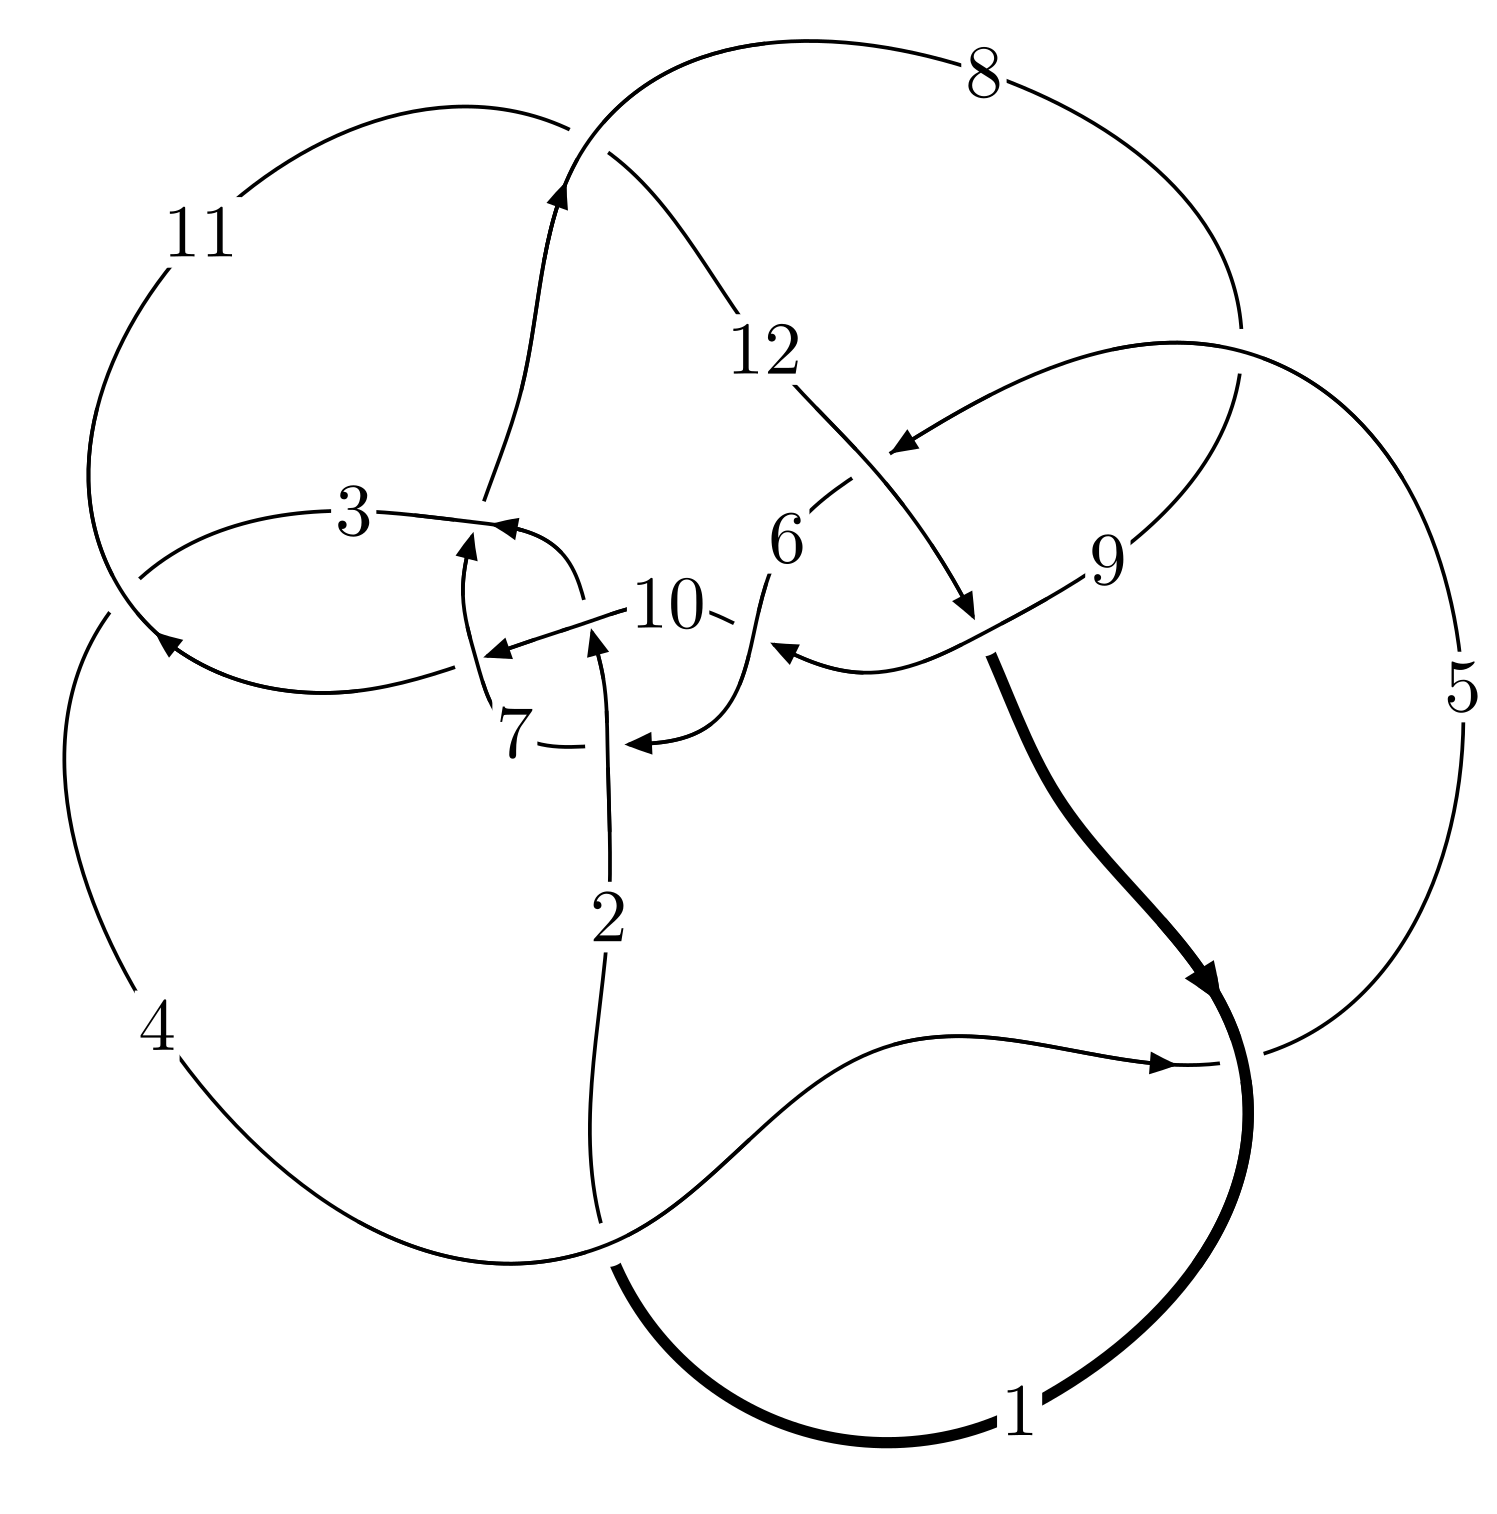
\includegraphics[width=112pt]{../../../GIT/diagram.site/Diagrams/png/1997_12a_1196.png}\\
\ \ \ A knot diagram\footnotemark}&
\allowdisplaybreaks
\textbf{Linearized knot diagam} \\
\cline{2-2}
 &
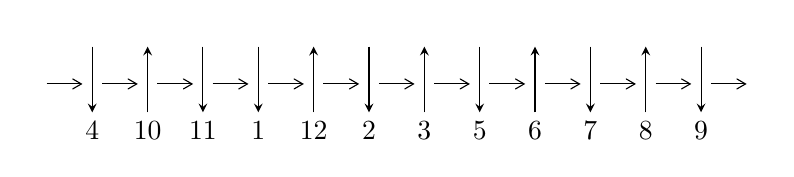
\begin{tikzpicture}[x=20pt, y=17pt]
	% nodes
	\node (C0) at (0, 0) {};
	\node (C1) at (1, 0) {};
	\node (C1U) at (1, +1) {};
	\node (C1D) at (1, -1) {4};

	\node (C2) at (2, 0) {};
	\node (C2U) at (2, +1) {};
	\node (C2D) at (2, -1) {10};

	\node (C3) at (3, 0) {};
	\node (C3U) at (3, +1) {};
	\node (C3D) at (3, -1) {11};

	\node (C4) at (4, 0) {};
	\node (C4U) at (4, +1) {};
	\node (C4D) at (4, -1) {1};

	\node (C5) at (5, 0) {};
	\node (C5U) at (5, +1) {};
	\node (C5D) at (5, -1) {12};

	\node (C6) at (6, 0) {};
	\node (C6U) at (6, +1) {};
	\node (C6D) at (6, -1) {2};

	\node (C7) at (7, 0) {};
	\node (C7U) at (7, +1) {};
	\node (C7D) at (7, -1) {3};

	\node (C8) at (8, 0) {};
	\node (C8U) at (8, +1) {};
	\node (C8D) at (8, -1) {5};

	\node (C9) at (9, 0) {};
	\node (C9U) at (9, +1) {};
	\node (C9D) at (9, -1) {6};

	\node (C10) at (10, 0) {};
	\node (C10U) at (10, +1) {};
	\node (C10D) at (10, -1) {7};

	\node (C11) at (11, 0) {};
	\node (C11U) at (11, +1) {};
	\node (C11D) at (11, -1) {8};

	\node (C12) at (12, 0) {};
	\node (C12U) at (12, +1) {};
	\node (C12D) at (12, -1) {9};
	\node (C13) at (13, 0) {};

	% arrows
	\draw[->,>={angle 60}]
	(C0) edge (C1) (C1) edge (C2) (C2) edge (C3) (C3) edge (C4) (C4) edge (C5) (C5) edge (C6) (C6) edge (C7) (C7) edge (C8) (C8) edge (C9) (C9) edge (C10) (C10) edge (C11) (C11) edge (C12) (C12) edge (C13) ;	\draw[->,>=stealth]
	(C1U) edge (C1D) (C2D) edge (C2U) (C3U) edge (C3D) (C4U) edge (C4D) (C5D) edge (C5U) (C6U) edge (C6D) (C7D) edge (C7U) (C8U) edge (C8D) (C9D) edge (C9U) (C10U) edge (C10D) (C11D) edge (C11U) (C12U) edge (C12D) ;
	\end{tikzpicture} \\
\hhline{~~} \\& 
\textbf{Solving Sequence} \\ \cline{2-2} 
 &
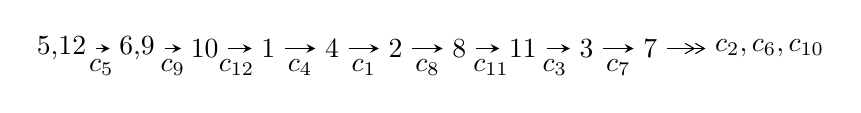
\begin{tikzpicture}[x=23pt, y=7pt]
	% node
	\node (A0) at (-1/8, 0) {5,12};
	\node (A1) at (17/16, 0) {6,9};
	\node (A2) at (17/8, 0) {10};
	\node (A3) at (25/8, 0) {1};
	\node (A4) at (33/8, 0) {4};
	\node (A5) at (41/8, 0) {2};
	\node (A6) at (49/8, 0) {8};
	\node (A7) at (57/8, 0) {11};
	\node (A8) at (65/8, 0) {3};
	\node (A9) at (73/8, 0) {7};
	\node (C1) at (1/2, -1) {$c_{5}$};
	\node (C2) at (13/8, -1) {$c_{9}$};
	\node (C3) at (21/8, -1) {$c_{12}$};
	\node (C4) at (29/8, -1) {$c_{4}$};
	\node (C5) at (37/8, -1) {$c_{1}$};
	\node (C6) at (45/8, -1) {$c_{8}$};
	\node (C7) at (53/8, -1) {$c_{11}$};
	\node (C8) at (61/8, -1) {$c_{3}$};
	\node (C9) at (69/8, -1) {$c_{7}$};
	\node (A10) at (11, 0) {$c_{2},c_{6},c_{10}$};

	% edge
	\draw[->,>=stealth]	
	(A0) edge (A1) (A1) edge (A2) (A2) edge (A3) (A3) edge (A4) (A4) edge (A5) (A5) edge (A6) (A6) edge (A7) (A7) edge (A8) (A8) edge (A9) ;
	\draw[->>,>={angle 60}]	
	(A9) edge (A10);
\end{tikzpicture} \\ 

\end{tabular} \\

\footnotetext{
The image of knot diagram is generated by the software ``\textbf{Draw programme}" developed by Andrew Bartholomew(\url{http://www.layer8.co.uk/maths/draw/index.htm\#Running-draw}), where we modified some parts for our purpose(\url{https://github.com/CATsTAILs/LinksPainter}).
}\phantom \\ \newline 
\centering \textbf{Ideals for irreducible components\footnotemark of $X_{\text{par}}$} 
 
\begin{align*}
I^u_{1}&=\langle 
1.08642\times10^{59} u^{46}-4.09896\times10^{60} u^{45}+\cdots+9.38798\times10^{59} b-4.54188\times10^{62},\\
\phantom{I^u_{1}}&\phantom{= \langle  }-1.10886\times10^{59} u^{46}+4.10726\times10^{60} u^{45}+\cdots+1.87760\times10^{60} a+2.91033\times10^{62},\\
\phantom{I^u_{1}}&\phantom{= \langle  }u^{47}-39 u^{46}+\cdots-102400 u+8192\rangle \\
I^u_{2}&=\langle 
-1.13339\times10^{29} u^{70}-4.82195\times10^{30} u^{69}+\cdots+4.88548\times10^{24} b+2.41929\times10^{31},\\
\phantom{I^u_{2}}&\phantom{= \langle  }-4.83859\times10^{30} a u^{70}-8.29715\times10^{30} u^{70}+\cdots+6.34635\times10^{31} a+6.92021\times10^{31},\\
\phantom{I^u_{2}}&\phantom{= \langle  }u^{71}+22 u^{70}+\cdots-55 u-5\rangle \\
I^u_{3}&=\langle 
2.16517\times10^{20} u^{30}+3.26536\times10^{21} u^{29}+\cdots+1.19902\times10^{21} b+2.70066\times10^{20},\\
\phantom{I^u_{3}}&\phantom{= \langle  }2.70066\times10^{20} u^{30}+3.72737\times10^{21} u^{29}+\cdots+1.19902\times10^{21} a+4.45709\times10^{21},\;u^{31}+13 u^{30}+\cdots+u-1\rangle \\
I^u_{4}&=\langle 
4 u^3+5 a u-11 u^2+5 b+17 u-11,\;11 u^3 a-24 u^2 a-6 u^3+25 a^2+33 a u+29 u^2-14 a-43 u+44,\\
\phantom{I^u_{4}}&\phantom{= \langle  }u^4-4 u^3+8 u^2-9 u+5\rangle \\
I^u_{5}&=\langle 
b- u+2,\;3 a+2 u-3,\;u^2-3 u+3\rangle \\
I^u_{6}&=\langle 
a u+b- u,\;a^2- a- u+1,\;u^2- u+1\rangle \\
\\
\end{align*}
\raggedright * 6 irreducible components of $\dim_{\mathbb{C}}=0$, with total 234 representations.\\
\footnotetext{All coefficients of polynomials are rational numbers. But the coefficients are sometimes approximated in decimal forms when there is not enough margin.}
\newpage
\renewcommand{\arraystretch}{1}
\centering \section*{I. $I^u_{1}= \langle 1.09\times10^{59} u^{46}-4.10\times10^{60} u^{45}+\cdots+9.39\times10^{59} b-4.54\times10^{62},\;-1.11\times10^{59} u^{46}+4.11\times10^{60} u^{45}+\cdots+1.88\times10^{60} a+2.91\times10^{62},\;u^{47}-39 u^{46}+\cdots-102400 u+8192 \rangle$}
\flushleft \textbf{(i) Arc colorings}\\
\begin{tabular}{m{7pt} m{180pt} m{7pt} m{180pt} }
\flushright $a_{5}=$&$\begin{pmatrix}1\\0\end{pmatrix}$ \\
\flushright $a_{12}=$&$\begin{pmatrix}0\\u\end{pmatrix}$ \\
\flushright $a_{6}=$&$\begin{pmatrix}1\\- u^2\end{pmatrix}$ \\
\flushright $a_{9}=$&$\begin{pmatrix}0.0590573 u^{46}-2.18751 u^{45}+\cdots+1965.57 u-155.003\\-0.115724 u^{46}+4.36618 u^{45}+\cdots-5892.46 u+483.797\end{pmatrix}$ \\
\flushright $a_{10}=$&$\begin{pmatrix}0.0904063 u^{46}-3.49531 u^{45}+\cdots+7439.50 u-619.221\\0.184438 u^{46}-6.83157 u^{45}+\cdots+3087.53 u-214.057\end{pmatrix}$ \\
\flushright $a_{1}=$&$\begin{pmatrix}0.0254493 u^{46}-0.964977 u^{45}+\cdots+1631.99 u-133.385\\-0.0275439 u^{46}+1.05235 u^{45}+\cdots-2471.62 u+208.480\end{pmatrix}$ \\
\flushright $a_{4}=$&$\begin{pmatrix}0.0448796 u^{46}-1.72346 u^{45}+\cdots+3562.00 u-289.190\\-0.00498553 u^{46}+0.226727 u^{45}+\cdots-1693.46 u+142.014\end{pmatrix}$ \\
\flushright $a_{2}=$&$\begin{pmatrix}-0.0169903 u^{46}+0.589287 u^{45}+\cdots+1838.44 u-163.476\\0.0629036 u^{46}-2.42072 u^{45}+\cdots+4884.80 u-405.666\end{pmatrix}$ \\
\flushright $a_{8}=$&$\begin{pmatrix}-0.0566672 u^{46}+2.17867 u^{45}+\cdots-3926.89 u+328.794\\-0.115724 u^{46}+4.36618 u^{45}+\cdots-5892.46 u+483.797\end{pmatrix}$ \\
\flushright $a_{11}=$&$\begin{pmatrix}-0.00777706 u^{46}+0.294739 u^{45}+\cdots-701.230 u+57.9358\\-0.00568240 u^{46}+0.207365 u^{45}+\cdots+140.398 u-17.1594\end{pmatrix}$ \\
\flushright $a_{3}=$&$\begin{pmatrix}-0.0481510 u^{46}+1.87081 u^{45}+\cdots-3664.83 u+303.197\\-0.132055 u^{46}+4.93655 u^{45}+\cdots-4297.19 u+336.475\end{pmatrix}$ \\
\flushright $a_{7}=$&$\begin{pmatrix}0.0320196 u^{46}-1.33035 u^{45}+\cdots+7164.01 u-616.138\\0.163583 u^{46}-6.19951 u^{45}+\cdots+8115.42 u-654.306\end{pmatrix}$\\&\end{tabular}
\flushleft \textbf{(ii) Obstruction class $= -1$}\\~\\
\flushleft \textbf{(iii) Cusp Shapes $= -0.0277438 u^{46}+0.925540 u^{45}+\cdots-1341.39 u+155.582$}\\~\\
\newpage\renewcommand{\arraystretch}{1}
\flushleft \textbf{(iv) u-Polynomials at the component}\newline \\
\begin{tabular}{m{50pt}|m{274pt}}
Crossings & \hspace{64pt}u-Polynomials at each crossing \\
\hline $$\begin{aligned}c_{1},c_{4}\end{aligned}$$&$\begin{aligned}
&u^{47}-23 u^{46}+\cdots-13056 u+1024
\end{aligned}$\\
\hline $$\begin{aligned}c_{2},c_{7}\end{aligned}$$&$\begin{aligned}
&u^{47}+3 u^{46}+\cdots+2 u+1
\end{aligned}$\\
\hline $$\begin{aligned}c_{3},c_{6}\end{aligned}$$&$\begin{aligned}
&u^{47}+2 u^{46}+\cdots-5 u+2
\end{aligned}$\\
\hline $$\begin{aligned}c_{5}\end{aligned}$$&$\begin{aligned}
&u^{47}-39 u^{46}+\cdots-102400 u+8192
\end{aligned}$\\
\hline $$\begin{aligned}c_{8},c_{12}\end{aligned}$$&$\begin{aligned}
&u^{47}+2 u^{46}+\cdots+12 u+1
\end{aligned}$\\
\hline $$\begin{aligned}c_{9},c_{11}\end{aligned}$$&$\begin{aligned}
&u^{47}- u^{46}+\cdots-1149 u+457
\end{aligned}$\\
\hline $$\begin{aligned}c_{10}\end{aligned}$$&$\begin{aligned}
&u^{47}+27 u^{46}+\cdots-608 u-32
\end{aligned}$\\
\hline
\end{tabular}\\~\\
\newpage\renewcommand{\arraystretch}{1}
\flushleft \textbf{(v) Riley Polynomials at the component}\newline \\
\begin{tabular}{m{50pt}|m{274pt}}
Crossings & \hspace{64pt}Riley Polynomials at each crossing \\
\hline $$\begin{aligned}c_{1},c_{4}\end{aligned}$$&$\begin{aligned}
&y^{47}+39 y^{46}+\cdots-19595264 y-1048576
\end{aligned}$\\
\hline $$\begin{aligned}c_{2},c_{7}\end{aligned}$$&$\begin{aligned}
&y^{47}-21 y^{46}+\cdots+40 y-1
\end{aligned}$\\
\hline $$\begin{aligned}c_{3},c_{6}\end{aligned}$$&$\begin{aligned}
&y^{47}+4 y^{46}+\cdots-67 y-4
\end{aligned}$\\
\hline $$\begin{aligned}c_{5}\end{aligned}$$&$\begin{aligned}
&y^{47}+y^{46}+\cdots-2097152000 y-67108864
\end{aligned}$\\
\hline $$\begin{aligned}c_{8},c_{12}\end{aligned}$$&$\begin{aligned}
&y^{47}+16 y^{46}+\cdots+60 y-1
\end{aligned}$\\
\hline $$\begin{aligned}c_{9},c_{11}\end{aligned}$$&$\begin{aligned}
&y^{47}-27 y^{46}+\cdots+3980855 y-208849
\end{aligned}$\\
\hline $$\begin{aligned}c_{10}\end{aligned}$$&$\begin{aligned}
&y^{47}+y^{46}+\cdots+18944 y-1024
\end{aligned}$\\
\hline
\end{tabular}\\~\\
\newpage\flushleft \textbf{(vi) Complex Volumes and Cusp Shapes}
$$\begin{array}{c|c|c}  
\text{Solutions to }I^u_{1}& \I (\text{vol} + \sqrt{-1}CS) & \text{Cusp shape}\\
 \hline 
\begin{aligned}
u &= \phantom{-}0.789858 + 0.572021 I \\
a &= \phantom{-}0.795254 + 0.602395 I \\
b &= -0.283556 - 0.930709 I\end{aligned}
 & \phantom{-}3.17145 + 1.69281 I & \phantom{-0.000000 } 0 \\ \hline\begin{aligned}
u &= \phantom{-}0.789858 - 0.572021 I \\
a &= \phantom{-}0.795254 - 0.602395 I \\
b &= -0.283556 + 0.930709 I\end{aligned}
 & \phantom{-}3.17145 - 1.69281 I & \phantom{-0.000000 } 0 \\ \hline\begin{aligned}
u &= \phantom{-}0.106416 + 1.060570 I \\
a &= -0.169028 - 0.771034 I \\
b &= -0.799746 + 0.261315 I\end{aligned}
 & -2.73254 - 6.81022 I & \phantom{-0.000000 } 0 \\ \hline\begin{aligned}
u &= \phantom{-}0.106416 - 1.060570 I \\
a &= -0.169028 + 0.771034 I \\
b &= -0.799746 - 0.261315 I\end{aligned}
 & -2.73254 + 6.81022 I & \phantom{-0.000000 } 0 \\ \hline\begin{aligned}
u &= \phantom{-}0.323409 + 1.054660 I \\
a &= \phantom{-}0.342192 + 0.658803 I \\
b &= \phantom{-}0.584148 - 0.573961 I\end{aligned}
 & -0.33944 + 1.43644 I & \phantom{-0.000000 } 0 \\ \hline\begin{aligned}
u &= \phantom{-}0.323409 - 1.054660 I \\
a &= \phantom{-}0.342192 - 0.658803 I \\
b &= \phantom{-}0.584148 + 0.573961 I\end{aligned}
 & -0.33944 - 1.43644 I & \phantom{-0.000000 } 0 \\ \hline\begin{aligned}
u &= \phantom{-}0.674599 + 0.980557 I \\
a &= \phantom{-}0.362289 + 1.183380 I \\
b &= \phantom{-}0.91597 - 1.15355 I\end{aligned}
 & \phantom{-}1.96072 + 3.71013 I & \phantom{-0.000000 } 0 \\ \hline\begin{aligned}
u &= \phantom{-}0.674599 - 0.980557 I \\
a &= \phantom{-}0.362289 - 1.183380 I \\
b &= \phantom{-}0.91597 + 1.15355 I\end{aligned}
 & \phantom{-}1.96072 - 3.71013 I & \phantom{-0.000000 } 0 \\ \hline\begin{aligned}
u &= \phantom{-}0.624716 + 0.471470 I \\
a &= \phantom{-}0.373351 + 1.327370 I \\
b &= \phantom{-}0.392576 - 1.005250 I\end{aligned}
 & \phantom{-}0.432423 + 1.337180 I & \phantom{-0.000000 } 0 \\ \hline\begin{aligned}
u &= \phantom{-}0.624716 - 0.471470 I \\
a &= \phantom{-}0.373351 - 1.327370 I \\
b &= \phantom{-}0.392576 + 1.005250 I\end{aligned}
 & \phantom{-}0.432423 - 1.337180 I & \phantom{-0.000000 } 0\\
 \hline 
 \end{array}$$\newpage$$\begin{array}{c|c|c}  
\text{Solutions to }I^u_{1}& \I (\text{vol} + \sqrt{-1}CS) & \text{Cusp shape}\\
 \hline 
\begin{aligned}
u &= \phantom{-}0.020792 + 0.725962 I \\
a &= \phantom{-}0.450343 + 1.201190 I \\
b &= \phantom{-}0.862651 - 0.351907 I\end{aligned}
 & -3.02055 + 2.57813 I & -8.49493 - 6.08362 I \\ \hline\begin{aligned}
u &= \phantom{-}0.020792 - 0.725962 I \\
a &= \phantom{-}0.450343 - 1.201190 I \\
b &= \phantom{-}0.862651 + 0.351907 I\end{aligned}
 & -3.02055 - 2.57813 I & -8.49493 + 6.08362 I \\ \hline\begin{aligned}
u &= -1.30541\phantom{ +0.000000I} \\
a &= \phantom{-}0.0836022\phantom{ +0.000000I} \\
b &= \phantom{-}0.109135\phantom{ +0.000000I}\end{aligned}
 & -2.49946\phantom{ +0.000000I} & \phantom{-0.000000 } 0 \\ \hline\begin{aligned}
u &= \phantom{-}0.298531 + 0.575032 I \\
a &= -0.34160 - 1.76890 I \\
b &= -0.915194 + 0.724506 I\end{aligned}
 & -2.40724 - 2.07518 I & -6.28983 + 0.97864 I \\ \hline\begin{aligned}
u &= \phantom{-}0.298531 - 0.575032 I \\
a &= -0.34160 + 1.76890 I \\
b &= -0.915194 - 0.724506 I\end{aligned}
 & -2.40724 + 2.07518 I & -6.28983 - 0.97864 I \\ \hline\begin{aligned}
u &= \phantom{-}1.210210 + 0.716417 I \\
a &= -0.093445 + 1.110070 I \\
b &= \phantom{-}0.90836 - 1.27648 I\end{aligned}
 & \phantom{-}10.14280 + 2.59316 I & \phantom{-0.000000 } 0 \\ \hline\begin{aligned}
u &= \phantom{-}1.210210 - 0.716417 I \\
a &= -0.093445 - 1.110070 I \\
b &= \phantom{-}0.90836 + 1.27648 I\end{aligned}
 & \phantom{-}10.14280 - 2.59316 I & \phantom{-0.000000 } 0 \\ \hline\begin{aligned}
u &= \phantom{-}0.016785 + 0.585660 I \\
a &= \phantom{-}0.708909 + 0.408464 I \\
b &= \phantom{-}0.227322 - 0.422036 I\end{aligned}
 & -0.136287 + 1.304410 I & -1.20224 - 5.79186 I \\ \hline\begin{aligned}
u &= \phantom{-}0.016785 - 0.585660 I \\
a &= \phantom{-}0.708909 - 0.408464 I \\
b &= \phantom{-}0.227322 + 0.422036 I\end{aligned}
 & -0.136287 - 1.304410 I & -1.20224 + 5.79186 I \\ \hline\begin{aligned}
u &= \phantom{-}0.025935 + 0.489011 I \\
a &= \phantom{-}1.60407 + 2.15189 I \\
b &= \phantom{-}1.010700 - 0.840218 I\end{aligned}
 & \phantom{-}0.30273 + 6.30888 I & -2.19256 - 11.23940 I\\
 \hline 
 \end{array}$$\newpage$$\begin{array}{c|c|c}  
\text{Solutions to }I^u_{1}& \I (\text{vol} + \sqrt{-1}CS) & \text{Cusp shape}\\
 \hline 
\begin{aligned}
u &= \phantom{-}0.025935 - 0.489011 I \\
a &= \phantom{-}1.60407 - 2.15189 I \\
b &= \phantom{-}1.010700 + 0.840218 I\end{aligned}
 & \phantom{-}0.30273 - 6.30888 I & -2.19256 + 11.23940 I \\ \hline\begin{aligned}
u &= \phantom{-}1.18191 + 0.97444 I \\
a &= -0.112442 - 1.005100 I \\
b &= -0.84651 + 1.29750 I\end{aligned}
 & \phantom{-}8.05895 + 6.03050 I & \phantom{-0.000000 } 0 \\ \hline\begin{aligned}
u &= \phantom{-}1.18191 - 0.97444 I \\
a &= -0.112442 + 1.005100 I \\
b &= -0.84651 - 1.29750 I\end{aligned}
 & \phantom{-}8.05895 - 6.03050 I & \phantom{-0.000000 } 0 \\ \hline\begin{aligned}
u &= \phantom{-}1.35978 + 0.81114 I \\
a &= \phantom{-}0.080566 - 0.958947 I \\
b &= -0.88739 + 1.23860 I\end{aligned}
 & \phantom{-}8.74035 + 7.98020 I & \phantom{-0.000000 } 0 \\ \hline\begin{aligned}
u &= \phantom{-}1.35978 - 0.81114 I \\
a &= \phantom{-}0.080566 + 0.958947 I \\
b &= -0.88739 - 1.23860 I\end{aligned}
 & \phantom{-}8.74035 - 7.98020 I & \phantom{-0.000000 } 0 \\ \hline\begin{aligned}
u &= \phantom{-}1.24199 + 1.08453 I \\
a &= \phantom{-}0.064228 + 0.996984 I \\
b &= \phantom{-}1.00149 - 1.30790 I\end{aligned}
 & \phantom{-}8.2473 + 21.8470 I & \phantom{-0.000000 } 0 \\ \hline\begin{aligned}
u &= \phantom{-}1.24199 - 1.08453 I \\
a &= \phantom{-}0.064228 - 0.996984 I \\
b &= \phantom{-}1.00149 + 1.30790 I\end{aligned}
 & \phantom{-}8.2473 - 21.8470 I & \phantom{-0.000000 } 0 \\ \hline\begin{aligned}
u &= \phantom{-}1.21311 + 1.14031 I \\
a &= -0.111952 - 0.975187 I \\
b &= -0.97621 + 1.31067 I\end{aligned}
 & \phantom{-}9.1579 + 13.1525 I & \phantom{-0.000000 } 0 \\ \hline\begin{aligned}
u &= \phantom{-}1.21311 - 1.14031 I \\
a &= -0.111952 + 0.975187 I \\
b &= -0.97621 - 1.31067 I\end{aligned}
 & \phantom{-}9.1579 - 13.1525 I & \phantom{-0.000000 } 0 \\ \hline\begin{aligned}
u &= -0.140578 + 0.193465 I \\
a &= \phantom{-}0.65556 - 4.39100 I \\
b &= -0.757348 - 0.744107 I\end{aligned}
 & \phantom{-}5.01435 + 2.53794 I & \phantom{-}0.84043 - 2.77896 I\\
 \hline 
 \end{array}$$\newpage$$\begin{array}{c|c|c}  
\text{Solutions to }I^u_{1}& \I (\text{vol} + \sqrt{-1}CS) & \text{Cusp shape}\\
 \hline 
\begin{aligned}
u &= -0.140578 - 0.193465 I \\
a &= \phantom{-}0.65556 + 4.39100 I \\
b &= -0.757348 + 0.744107 I\end{aligned}
 & \phantom{-}5.01435 - 2.53794 I & \phantom{-}0.84043 + 2.77896 I \\ \hline\begin{aligned}
u &= \phantom{-}1.15618 + 1.33193 I \\
a &= -0.360678 - 0.340815 I \\
b &= -0.036934 + 0.874442 I\end{aligned}
 & \phantom{-}7.12799 + 2.40033 I & \phantom{-0.000000 } 0 \\ \hline\begin{aligned}
u &= \phantom{-}1.15618 - 1.33193 I \\
a &= -0.360678 + 0.340815 I \\
b &= -0.036934 - 0.874442 I\end{aligned}
 & \phantom{-}7.12799 - 2.40033 I & \phantom{-0.000000 } 0 \\ \hline\begin{aligned}
u &= \phantom{-}1.31536 + 1.18518 I \\
a &= -0.033298 - 0.670801 I \\
b &= -0.751219 + 0.921810 I\end{aligned}
 & \phantom{-}4.06199 + 7.90337 I & \phantom{-0.000000 } 0 \\ \hline\begin{aligned}
u &= \phantom{-}1.31536 - 1.18518 I \\
a &= -0.033298 + 0.670801 I \\
b &= -0.751219 - 0.921810 I\end{aligned}
 & \phantom{-}4.06199 - 7.90337 I & \phantom{-0.000000 } 0 \\ \hline\begin{aligned}
u &= \phantom{-}1.43565 + 1.13278 I \\
a &= -0.070763 + 0.656697 I \\
b &= \phantom{-}0.845485 - 0.862632 I\end{aligned}
 & \phantom{-}2.4290 + 15.1963 I & \phantom{-0.000000 } 0 \\ \hline\begin{aligned}
u &= \phantom{-}1.43565 - 1.13278 I \\
a &= -0.070763 - 0.656697 I \\
b &= \phantom{-}0.845485 + 0.862632 I\end{aligned}
 & \phantom{-}2.4290 - 15.1963 I & \phantom{-0.000000 } 0 \\ \hline\begin{aligned}
u &= \phantom{-}1.71474 + 0.65476 I \\
a &= -0.178004 + 0.533259 I \\
b &= \phantom{-}0.654385 - 0.797849 I\end{aligned}
 & \phantom{-}3.38591 - 3.98691 I & \phantom{-0.000000 } 0 \\ \hline\begin{aligned}
u &= \phantom{-}1.71474 - 0.65476 I \\
a &= -0.178004 - 0.533259 I \\
b &= \phantom{-}0.654385 + 0.797849 I\end{aligned}
 & \phantom{-}3.38591 + 3.98691 I & \phantom{-0.000000 } 0 \\ \hline\begin{aligned}
u &= \phantom{-}1.47478 + 1.21882 I \\
a &= -0.363781 - 0.353820 I \\
b &= \phantom{-}0.105251 + 0.965191 I\end{aligned}
 & \phantom{-}9.18769 - 3.84376 I & \phantom{-0.000000 } 0\\
 \hline 
 \end{array}$$\newpage$$\begin{array}{c|c|c}  
\text{Solutions to }I^u_{1}& \I (\text{vol} + \sqrt{-1}CS) & \text{Cusp shape}\\
 \hline 
\begin{aligned}
u &= \phantom{-}1.47478 - 1.21882 I \\
a &= -0.363781 + 0.353820 I \\
b &= \phantom{-}0.105251 - 0.965191 I\end{aligned}
 & \phantom{-}9.18769 + 3.84376 I & \phantom{-0.000000 } 0 \\ \hline\begin{aligned}
u &= \phantom{-}1.44593 + 1.42503 I \\
a &= \phantom{-}0.343723 + 0.269068 I \\
b &= -0.113569 - 0.878869 I\end{aligned}
 & \phantom{-}7.6878 - 12.4770 I & \phantom{-0.000000 } 0 \\ \hline\begin{aligned}
u &= \phantom{-}1.44593 - 1.42503 I \\
a &= \phantom{-}0.343723 - 0.269068 I \\
b &= -0.113569 + 0.878869 I\end{aligned}
 & \phantom{-}7.6878 + 12.4770 I & \phantom{-0.000000 } 0 \\ \hline\begin{aligned}
u &= \phantom{-}1.58102 + 1.61441 I \\
a &= -0.142057 - 0.292779 I \\
b &= -0.248071 + 0.692228 I\end{aligned}
 & \phantom{-}6.42396 + 1.69767 I & \phantom{-0.000000 } 0 \\ \hline\begin{aligned}
u &= \phantom{-}1.58102 - 1.61441 I \\
a &= -0.142057 + 0.292779 I \\
b &= -0.248071 - 0.692228 I\end{aligned}
 & \phantom{-}6.42396 - 1.69767 I & \phantom{-0.000000 } 0 \\ \hline\begin{aligned}
u &= \phantom{-}1.08159 + 2.43719 I \\
a &= \phantom{-}0.154769 + 0.090366 I \\
b &= \phantom{-}0.052843 - 0.474939 I\end{aligned}
 & \phantom{-}6.46891 + 5.45398 I & \phantom{-0.000000 } 0 \\ \hline\begin{aligned}
u &= \phantom{-}1.08159 - 2.43719 I \\
a &= \phantom{-}0.154769 - 0.090366 I \\
b &= \phantom{-}0.052843 + 0.474939 I\end{aligned}
 & \phantom{-}6.46891 - 5.45398 I & \phantom{-0.000000 } 0\\
 \hline 
 \end{array}$$\newpage\newpage\renewcommand{\arraystretch}{1}
\centering \section*{II. $I^u_{2}= \langle -1.13\times10^{29} u^{70}-4.82\times10^{30} u^{69}+\cdots+4.89\times10^{24} b+2.42\times10^{31},\;-4.84\times10^{30} a u^{70}-8.30\times10^{30} u^{70}+\cdots+6.35\times10^{31} a+6.92\times10^{31},\;u^{71}+22 u^{70}+\cdots-55 u-5 \rangle$}
\flushleft \textbf{(i) Arc colorings}\\
\begin{tabular}{m{7pt} m{180pt} m{7pt} m{180pt} }
\flushright $a_{5}=$&$\begin{pmatrix}1\\0\end{pmatrix}$ \\
\flushright $a_{12}=$&$\begin{pmatrix}0\\u\end{pmatrix}$ \\
\flushright $a_{6}=$&$\begin{pmatrix}1\\- u^2\end{pmatrix}$ \\
\flushright $a_{9}=$&$\begin{pmatrix}a\\23199.1 u^{70}+986996. u^{69}+\cdots-4.14818\times10^{7} u-4.95200\times10^{6}\end{pmatrix}$ \\
\flushright $a_{10}=$&$\begin{pmatrix}23199.1 u^{70}+986996. u^{69}+\cdots+a-4.95200\times10^{6}\\687394. u^{70}+1.49354\times10^{7} u^{69}+\cdots-6.78117\times10^{7} u-7.33508\times10^{6}\end{pmatrix}$ \\
\flushright $a_{1}=$&$\begin{pmatrix}23199.1 a u^{70}+867570. u^{70}+\cdots-4.95200\times10^{6} a-8.49164\times10^{6}\\-302197. u^{70}-6.69779\times10^{6} u^{69}+\cdots+3.92247\times10^{7} u+4.33785\times10^{6}\end{pmatrix}$ \\
\flushright $a_{4}=$&$\begin{pmatrix}-239938. a u^{70}-2.17987\times10^{6} u^{70}+\cdots-374469. a+1.84264\times10^{7}\\1.15630\times10^{6} u^{70}+2.48006\times10^{7} u^{69}+\cdots-8.91836\times10^{7} u-9.38837\times10^{6}\end{pmatrix}$ \\
\flushright $a_{2}=$&$\begin{pmatrix}-2.31944\times10^{6} a u^{70}+3.07476\times10^{6} u^{70}+\cdots+1.54147\times10^{7} a-2.27294\times10^{7}\\-1.34228\times10^{6} u^{70}-2.84842\times10^{7} u^{69}+\cdots+7.98915\times10^{7} u+8.08133\times10^{6}\end{pmatrix}$ \\
\flushright $a_{8}=$&$\begin{pmatrix}23199.1 u^{70}+986996. u^{69}+\cdots+a-4.95200\times10^{6}\\23199.1 u^{70}+986996. u^{69}+\cdots-4.14818\times10^{7} u-4.95200\times10^{6}\end{pmatrix}$ \\
\flushright $a_{11}=$&$\begin{pmatrix}687394. a u^{70}+676175. u^{70}+\cdots-7.33508\times10^{6} a-6.73339\times10^{6}\\664195. a u^{70}+110802. u^{70}+\cdots-2.38308\times10^{6} a-2.57961\times10^{6}\end{pmatrix}$ \\
\flushright $a_{3}=$&$\begin{pmatrix}373244. a u^{70}-2.32863\times10^{6} u^{70}+\cdots+1.90152\times10^{6} a+9.68437\times10^{6}\\-152067. a u^{70}-1.85415\times10^{6} u^{70}+\cdots+2.01714\times10^{6} a+1.32832\times10^{7}\end{pmatrix}$ \\
\flushright $a_{7}=$&$\begin{pmatrix}288778. a u^{70}+1.33982\times10^{6} u^{70}+\cdots-528893. a-6.61449\times10^{6}\\-909066. a u^{70}+877015. u^{70}+\cdots+5.32274\times10^{6} a-4.34410\times10^{6}\end{pmatrix}$\\&\end{tabular}
\flushleft \textbf{(ii) Obstruction class $= -1$}\\~\\
\flushleft \textbf{(iii) Cusp Shapes $= \frac{6672500342500645145827521018811}{1221371038010135829969920} u^{70}+\frac{70712871267280814406090494060611}{610685519005067914984960} u^{69}+\cdots-\frac{382511550256794372990851752886051}{1221371038010135829969920} u-\frac{119784397586000680545676883339}{3816784493781674468656}$}\\~\\
\newpage\renewcommand{\arraystretch}{1}
\flushleft \textbf{(iv) u-Polynomials at the component}\newline \\
\begin{tabular}{m{50pt}|m{274pt}}
Crossings & \hspace{64pt}u-Polynomials at each crossing \\
\hline $$\begin{aligned}c_{1}\end{aligned}$$&$\begin{aligned}
&(u^{71}+14 u^{70}+\cdots+566 u+148)^{2}
\end{aligned}$\\
\hline $$\begin{aligned}c_{2}\end{aligned}$$&$\begin{aligned}
&5 u^{142}+30 u^{141}+\cdots+167385 u-47185
\end{aligned}$\\
\hline $$\begin{aligned}c_{3}\end{aligned}$$&$\begin{aligned}
&5 u^{142}+30 u^{141}+\cdots+6145 u+1339
\end{aligned}$\\
\hline $$\begin{aligned}c_{4}\end{aligned}$$&$\begin{aligned}
&(u^{71}-14 u^{70}+\cdots+566 u-148)^{2}
\end{aligned}$\\
\hline $$\begin{aligned}c_{5}\end{aligned}$$&$\begin{aligned}
&(u^{71}+22 u^{70}+\cdots-55 u-5)^{2}
\end{aligned}$\\
\hline $$\begin{aligned}c_{6}\end{aligned}$$&$\begin{aligned}
&5 u^{142}-30 u^{141}+\cdots-6145 u+1339
\end{aligned}$\\
\hline $$\begin{aligned}c_{7}\end{aligned}$$&$\begin{aligned}
&-5 u^{142}+30 u^{141}+\cdots+167385 u+47185
\end{aligned}$\\
\hline $$\begin{aligned}c_{8},c_{12}\end{aligned}$$&$\begin{aligned}
&-5 u^{142}+20 u^{141}+\cdots+4314935 u+821335
\end{aligned}$\\
\hline $$\begin{aligned}c_{9},c_{11}\end{aligned}$$&$\begin{aligned}
&-5 u^{142}+10 u^{141}+\cdots-271556615523 u+71833666691
\end{aligned}$\\
\hline $$\begin{aligned}c_{10}\end{aligned}$$&$\begin{aligned}
&(u^{71}+15 u^{70}+\cdots+65 u+5)^{2}
\end{aligned}$\\
\hline
\end{tabular}\\~\\
\newpage\renewcommand{\arraystretch}{1}
\flushleft \textbf{(v) Riley Polynomials at the component}\newline \\
\begin{tabular}{m{50pt}|m{274pt}}
Crossings & \hspace{64pt}Riley Polynomials at each crossing \\
\hline $$\begin{aligned}c_{1},c_{4}\end{aligned}$$&$\begin{aligned}
&(y^{71}+62 y^{70}+\cdots+341964 y-21904)^{2}
\end{aligned}$\\
\hline $$\begin{aligned}c_{2},c_{7}\end{aligned}$$&$\begin{aligned}
&25 y^{142}-410 y^{141}+\cdots-130716079465 y+2226424225
\end{aligned}$\\
\hline $$\begin{aligned}c_{3},c_{6}\end{aligned}$$&$\begin{aligned}
&25 y^{142}-60 y^{141}+\cdots-31957799 y+1792921
\end{aligned}$\\
\hline $$\begin{aligned}c_{5}\end{aligned}$$&$\begin{aligned}
&(y^{71}-12 y^{70}+\cdots+1515 y-25)^{2}
\end{aligned}$\\
\hline $$\begin{aligned}c_{8},c_{12}\end{aligned}$$&$\begin{aligned}
&25 y^{142}+510 y^{141}+\cdots+15566082199365 y+674591182225
\end{aligned}$\\
\hline $$\begin{aligned}c_{9},c_{11}\end{aligned}$$&$\begin{aligned}
&25 y^{142}-2240 y^{141}+\cdots-3.06\times10^{23} y+5.16\times10^{21}
\end{aligned}$\\
\hline $$\begin{aligned}c_{10}\end{aligned}$$&$\begin{aligned}
&(y^{71}-7 y^{70}+\cdots+1665 y-25)^{2}
\end{aligned}$\\
\hline
\end{tabular}\\~\\
\newpage\flushleft \textbf{(vi) Complex Volumes and Cusp Shapes}
$$\begin{array}{c|c|c}  
\text{Solutions to }I^u_{2}& \I (\text{vol} + \sqrt{-1}CS) & \text{Cusp shape}\\
 \hline 
\begin{aligned}
u &= -0.824672 + 0.570478 I \\
a &= -0.187954 - 1.090550 I \\
b &= \phantom{-}0.984144 + 0.902469 I\end{aligned}
 & -1.74041 - 5.49672 I & \phantom{-0.000000 } 0 \\ \hline\begin{aligned}
u &= -0.824672 + 0.570478 I \\
a &= \phantom{-}0.295125 + 1.298490 I \\
b &= -0.777137 - 0.792124 I\end{aligned}
 & -1.74041 - 5.49672 I & \phantom{-0.000000 } 0 \\ \hline\begin{aligned}
u &= -0.824672 - 0.570478 I \\
a &= -0.187954 + 1.090550 I \\
b &= \phantom{-}0.984144 - 0.902469 I\end{aligned}
 & -1.74041 + 5.49672 I & \phantom{-0.000000 } 0 \\ \hline\begin{aligned}
u &= -0.824672 - 0.570478 I \\
a &= \phantom{-}0.295125 - 1.298490 I \\
b &= -0.777137 + 0.792124 I\end{aligned}
 & -1.74041 + 5.49672 I & \phantom{-0.000000 } 0 \\ \hline\begin{aligned}
u &= -0.653521 + 0.738689 I \\
a &= \phantom{-}1.138200 + 0.225871 I \\
b &= -0.017427 + 0.499635 I\end{aligned}
 & \phantom{-}0.87960 + 2.11142 I & \phantom{-0.000000 } 0 \\ \hline\begin{aligned}
u &= -0.653521 + 0.738689 I \\
a &= -0.391121 + 0.322434 I \\
b &= \phantom{-}0.910684 - 0.693164 I\end{aligned}
 & \phantom{-}0.87960 + 2.11142 I & \phantom{-0.000000 } 0 \\ \hline\begin{aligned}
u &= -0.653521 - 0.738689 I \\
a &= \phantom{-}1.138200 - 0.225871 I \\
b &= -0.017427 - 0.499635 I\end{aligned}
 & \phantom{-}0.87960 - 2.11142 I & \phantom{-0.000000 } 0 \\ \hline\begin{aligned}
u &= -0.653521 - 0.738689 I \\
a &= -0.391121 - 0.322434 I \\
b &= \phantom{-}0.910684 + 0.693164 I\end{aligned}
 & \phantom{-}0.87960 - 2.11142 I & \phantom{-0.000000 } 0 \\ \hline\begin{aligned}
u &= -0.659920 + 0.791144 I \\
a &= \phantom{-}0.243572 + 0.702275 I \\
b &= -0.464563 - 0.227238 I\end{aligned}
 & -2.77623 + 0.61894 I & \phantom{-0.000000 } 0 \\ \hline\begin{aligned}
u &= -0.659920 + 0.791144 I \\
a &= -0.119461 - 0.487558 I \\
b &= \phantom{-}0.716339 + 0.270745 I\end{aligned}
 & -2.77623 + 0.61894 I & \phantom{-0.000000 } 0\\
 \hline 
 \end{array}$$\newpage$$\begin{array}{c|c|c}  
\text{Solutions to }I^u_{2}& \I (\text{vol} + \sqrt{-1}CS) & \text{Cusp shape}\\
 \hline 
\begin{aligned}
u &= -0.659920 - 0.791144 I \\
a &= \phantom{-}0.243572 - 0.702275 I \\
b &= -0.464563 + 0.227238 I\end{aligned}
 & -2.77623 - 0.61894 I & \phantom{-0.000000 } 0 \\ \hline\begin{aligned}
u &= -0.659920 - 0.791144 I \\
a &= -0.119461 + 0.487558 I \\
b &= \phantom{-}0.716339 - 0.270745 I\end{aligned}
 & -2.77623 - 0.61894 I & \phantom{-0.000000 } 0 \\ \hline\begin{aligned}
u &= \phantom{-}0.965142 + 0.087688 I \\
a &= \phantom{-}0.185351 - 0.854460 I \\
b &= -1.27250 + 1.58375 I\end{aligned}
 & \phantom{-}8.87060 - 1.96256 I & \phantom{-0.000000 } 0 \\ \hline\begin{aligned}
u &= \phantom{-}0.965142 + 0.087688 I \\
a &= \phantom{-}1.15979 - 1.74633 I \\
b &= -0.253816 + 0.808422 I\end{aligned}
 & \phantom{-}8.87060 - 1.96256 I & \phantom{-0.000000 } 0 \\ \hline\begin{aligned}
u &= \phantom{-}0.965142 - 0.087688 I \\
a &= \phantom{-}0.185351 + 0.854460 I \\
b &= -1.27250 - 1.58375 I\end{aligned}
 & \phantom{-}8.87060 + 1.96256 I & \phantom{-0.000000 } 0 \\ \hline\begin{aligned}
u &= \phantom{-}0.965142 - 0.087688 I \\
a &= \phantom{-}1.15979 + 1.74633 I \\
b &= -0.253816 - 0.808422 I\end{aligned}
 & \phantom{-}8.87060 + 1.96256 I & \phantom{-0.000000 } 0 \\ \hline\begin{aligned}
u &= -0.306428 + 0.912839 I \\
a &= \phantom{-}1.051020 - 0.593590 I \\
b &= \phantom{-}0.535534 + 0.082446 I\end{aligned}
 & \phantom{-}0.005444 + 0.532261 I & \phantom{-0.000000 } 0 \\ \hline\begin{aligned}
u &= -0.306428 + 0.912839 I \\
a &= \phantom{-}0.095820 + 0.554503 I \\
b &= -0.219791 - 1.141300 I\end{aligned}
 & \phantom{-}0.005444 + 0.532261 I & \phantom{-0.000000 } 0 \\ \hline\begin{aligned}
u &= -0.306428 - 0.912839 I \\
a &= \phantom{-}1.051020 + 0.593590 I \\
b &= \phantom{-}0.535534 - 0.082446 I\end{aligned}
 & \phantom{-}0.005444 - 0.532261 I & \phantom{-0.000000 } 0 \\ \hline\begin{aligned}
u &= -0.306428 - 0.912839 I \\
a &= \phantom{-}0.095820 - 0.554503 I \\
b &= -0.219791 + 1.141300 I\end{aligned}
 & \phantom{-}0.005444 - 0.532261 I & \phantom{-0.000000 } 0\\
 \hline 
 \end{array}$$\newpage$$\begin{array}{c|c|c}  
\text{Solutions to }I^u_{2}& \I (\text{vol} + \sqrt{-1}CS) & \text{Cusp shape}\\
 \hline 
\begin{aligned}
u &= \phantom{-}0.856259 + 0.418034 I \\
a &= \phantom{-}0.199182 + 1.016330 I \\
b &= -0.591258 - 0.801688 I\end{aligned}
 & \phantom{-}3.10625 + 2.38586 I & \phantom{-0.000000 } 0 \\ \hline\begin{aligned}
u &= \phantom{-}0.856259 + 0.418034 I \\
a &= \phantom{-}0.926724 + 0.483832 I \\
b &= \phantom{-}0.254309 - 0.953507 I\end{aligned}
 & \phantom{-}3.10625 + 2.38586 I & \phantom{-0.000000 } 0 \\ \hline\begin{aligned}
u &= \phantom{-}0.856259 - 0.418034 I \\
a &= \phantom{-}0.199182 - 1.016330 I \\
b &= -0.591258 + 0.801688 I\end{aligned}
 & \phantom{-}3.10625 - 2.38586 I & \phantom{-0.000000 } 0 \\ \hline\begin{aligned}
u &= \phantom{-}0.856259 - 0.418034 I \\
a &= \phantom{-}0.926724 - 0.483832 I \\
b &= \phantom{-}0.254309 + 0.953507 I\end{aligned}
 & \phantom{-}3.10625 - 2.38586 I & \phantom{-0.000000 } 0 \\ \hline\begin{aligned}
u &= -0.668333 + 0.630821 I \\
a &= \phantom{-}0.244078 + 1.244820 I \\
b &= -0.467567 - 0.406289 I\end{aligned}
 & -2.52859 - 2.05067 I & \phantom{-0.000000 } 0 \\ \hline\begin{aligned}
u &= -0.668333 + 0.630821 I \\
a &= -0.066534 - 0.670714 I \\
b &= \phantom{-}0.948385 + 0.677987 I\end{aligned}
 & -2.52859 - 2.05067 I & \phantom{-0.000000 } 0 \\ \hline\begin{aligned}
u &= -0.668333 - 0.630821 I \\
a &= \phantom{-}0.244078 - 1.244820 I \\
b &= -0.467567 + 0.406289 I\end{aligned}
 & -2.52859 + 2.05067 I & \phantom{-0.000000 } 0 \\ \hline\begin{aligned}
u &= -0.668333 - 0.630821 I \\
a &= -0.066534 + 0.670714 I \\
b &= \phantom{-}0.948385 - 0.677987 I\end{aligned}
 & -2.52859 + 2.05067 I & \phantom{-0.000000 } 0 \\ \hline\begin{aligned}
u &= -0.734328 + 0.551761 I \\
a &= -0.190018 - 1.142270 I \\
b &= \phantom{-}0.95657 + 1.47779 I\end{aligned}
 & \phantom{-}1.68399 - 6.46953 I & \phantom{-0.000000 } 0 \\ \hline\begin{aligned}
u &= -0.734328 + 0.551761 I \\
a &= -0.13388 + 1.91184 I \\
b &= -0.769797 - 0.733958 I\end{aligned}
 & \phantom{-}1.68399 - 6.46953 I & \phantom{-0.000000 } 0\\
 \hline 
 \end{array}$$\newpage$$\begin{array}{c|c|c}  
\text{Solutions to }I^u_{2}& \I (\text{vol} + \sqrt{-1}CS) & \text{Cusp shape}\\
 \hline 
\begin{aligned}
u &= -0.734328 - 0.551761 I \\
a &= -0.190018 + 1.142270 I \\
b &= \phantom{-}0.95657 - 1.47779 I\end{aligned}
 & \phantom{-}1.68399 + 6.46953 I & \phantom{-0.000000 } 0 \\ \hline\begin{aligned}
u &= -0.734328 - 0.551761 I \\
a &= -0.13388 - 1.91184 I \\
b &= -0.769797 + 0.733958 I\end{aligned}
 & \phantom{-}1.68399 + 6.46953 I & \phantom{-0.000000 } 0 \\ \hline\begin{aligned}
u &= -0.602775 + 0.959248 I \\
a &= \phantom{-}0.079718 + 1.096290 I \\
b &= -0.46599 - 1.72736 I\end{aligned}
 & \phantom{-}2.80463 - 0.98712 I & \phantom{-0.000000 } 0 \\ \hline\begin{aligned}
u &= -0.602775 + 0.959248 I \\
a &= \phantom{-}1.07214 - 1.15950 I \\
b &= \phantom{-}1.099670 + 0.584349 I\end{aligned}
 & \phantom{-}2.80463 - 0.98712 I & \phantom{-0.000000 } 0 \\ \hline\begin{aligned}
u &= -0.602775 - 0.959248 I \\
a &= \phantom{-}0.079718 - 1.096290 I \\
b &= -0.46599 + 1.72736 I\end{aligned}
 & \phantom{-}2.80463 + 0.98712 I & \phantom{-0.000000 } 0 \\ \hline\begin{aligned}
u &= -0.602775 - 0.959248 I \\
a &= \phantom{-}1.07214 + 1.15950 I \\
b &= \phantom{-}1.099670 - 0.584349 I\end{aligned}
 & \phantom{-}2.80463 + 0.98712 I & \phantom{-0.000000 } 0 \\ \hline\begin{aligned}
u &= \phantom{-}0.626316 + 0.977766 I \\
a &= -0.070814 - 1.063810 I \\
b &= -0.87454 + 1.62900 I\end{aligned}
 & \phantom{-}2.24238 + 12.49280 I & \phantom{-0.000000 } 0 \\ \hline\begin{aligned}
u &= \phantom{-}0.626316 + 0.977766 I \\
a &= -0.77508 - 1.39091 I \\
b &= -0.995807 + 0.735522 I\end{aligned}
 & \phantom{-}2.24238 + 12.49280 I & \phantom{-0.000000 } 0 \\ \hline\begin{aligned}
u &= \phantom{-}0.626316 - 0.977766 I \\
a &= -0.070814 + 1.063810 I \\
b &= -0.87454 - 1.62900 I\end{aligned}
 & \phantom{-}2.24238 - 12.49280 I & \phantom{-0.000000 } 0 \\ \hline\begin{aligned}
u &= \phantom{-}0.626316 - 0.977766 I \\
a &= -0.77508 + 1.39091 I \\
b &= -0.995807 - 0.735522 I\end{aligned}
 & \phantom{-}2.24238 - 12.49280 I & \phantom{-0.000000 } 0\\
 \hline 
 \end{array}$$\newpage$$\begin{array}{c|c|c}  
\text{Solutions to }I^u_{2}& \I (\text{vol} + \sqrt{-1}CS) & \text{Cusp shape}\\
 \hline 
\begin{aligned}
u &= -0.766108 + 0.227199 I \\
a &= \phantom{-}0.146877 - 0.712508 I \\
b &= -1.83837 + 1.33856 I\end{aligned}
 & \phantom{-}7.41218 - 3.70027 I & \phantom{-0.000000 } 0 \\ \hline\begin{aligned}
u &= -0.766108 + 0.227199 I \\
a &= -2.68191 + 0.95186 I \\
b &= -0.049357 - 0.579228 I\end{aligned}
 & \phantom{-}7.41218 - 3.70027 I & \phantom{-0.000000 } 0 \\ \hline\begin{aligned}
u &= -0.766108 - 0.227199 I \\
a &= \phantom{-}0.146877 + 0.712508 I \\
b &= -1.83837 - 1.33856 I\end{aligned}
 & \phantom{-}7.41218 + 3.70027 I & \phantom{-0.000000 } 0 \\ \hline\begin{aligned}
u &= -0.766108 - 0.227199 I \\
a &= -2.68191 - 0.95186 I \\
b &= -0.049357 + 0.579228 I\end{aligned}
 & \phantom{-}7.41218 + 3.70027 I & \phantom{-0.000000 } 0 \\ \hline\begin{aligned}
u &= -0.727284 + 0.202634 I \\
a &= \phantom{-}0.717941 + 1.218260 I \\
b &= \phantom{-}0.680119 - 1.113870 I\end{aligned}
 & \phantom{-}3.12602 - 9.03029 I & \phantom{-0.000000 } 0 \\ \hline\begin{aligned}
u &= -0.727284 + 0.202634 I \\
a &= \phantom{-}1.26376 - 1.17944 I \\
b &= \phantom{-}0.769008 + 0.740539 I\end{aligned}
 & \phantom{-}3.12602 - 9.03029 I & \phantom{-0.000000 } 0 \\ \hline\begin{aligned}
u &= -0.727284 - 0.202634 I \\
a &= \phantom{-}0.717941 - 1.218260 I \\
b &= \phantom{-}0.680119 + 1.113870 I\end{aligned}
 & \phantom{-}3.12602 + 9.03029 I & \phantom{-0.000000 } 0 \\ \hline\begin{aligned}
u &= -0.727284 - 0.202634 I \\
a &= \phantom{-}1.26376 + 1.17944 I \\
b &= \phantom{-}0.769008 - 0.740539 I\end{aligned}
 & \phantom{-}3.12602 + 9.03029 I & \phantom{-0.000000 } 0 \\ \hline\begin{aligned}
u &= \phantom{-}0.652637 + 1.074260 I \\
a &= -0.300909 - 1.021020 I \\
b &= -0.575617 + 0.453549 I\end{aligned}
 & -1.57416 + 8.84284 I & \phantom{-0.000000 } 0 \\ \hline\begin{aligned}
u &= \phantom{-}0.652637 + 1.074260 I \\
a &= -0.070610 - 0.578722 I \\
b &= -0.900458 + 0.989609 I\end{aligned}
 & -1.57416 + 8.84284 I & \phantom{-0.000000 } 0\\
 \hline 
 \end{array}$$\newpage$$\begin{array}{c|c|c}  
\text{Solutions to }I^u_{2}& \I (\text{vol} + \sqrt{-1}CS) & \text{Cusp shape}\\
 \hline 
\begin{aligned}
u &= \phantom{-}0.652637 - 1.074260 I \\
a &= -0.300909 + 1.021020 I \\
b &= -0.575617 - 0.453549 I\end{aligned}
 & -1.57416 - 8.84284 I & \phantom{-0.000000 } 0 \\ \hline\begin{aligned}
u &= \phantom{-}0.652637 - 1.074260 I \\
a &= -0.070610 + 0.578722 I \\
b &= -0.900458 - 0.989609 I\end{aligned}
 & -1.57416 - 8.84284 I & \phantom{-0.000000 } 0 \\ \hline\begin{aligned}
u &= -0.715680 + 0.181290 I \\
a &= -0.103054 + 0.864086 I \\
b &= \phantom{-}1.85725 - 1.31818 I\end{aligned}
 & \phantom{-}6.62178 - 12.35120 I & \phantom{-0.000000 } 0 \\ \hline\begin{aligned}
u &= -0.715680 + 0.181290 I \\
a &= \phantom{-}2.87704 - 1.11307 I \\
b &= \phantom{-}0.082896 + 0.637092 I\end{aligned}
 & \phantom{-}6.62178 - 12.35120 I & \phantom{-0.000000 } 0 \\ \hline\begin{aligned}
u &= -0.715680 - 0.181290 I \\
a &= -0.103054 - 0.864086 I \\
b &= \phantom{-}1.85725 + 1.31818 I\end{aligned}
 & \phantom{-}6.62178 + 12.35120 I & \phantom{-0.000000 } 0 \\ \hline\begin{aligned}
u &= -0.715680 - 0.181290 I \\
a &= \phantom{-}2.87704 + 1.11307 I \\
b &= \phantom{-}0.082896 - 0.637092 I\end{aligned}
 & \phantom{-}6.62178 + 12.35120 I & \phantom{-0.000000 } 0 \\ \hline\begin{aligned}
u &= -0.692516 + 0.244640 I \\
a &= \phantom{-}0.069672 - 1.247530 I \\
b &= \phantom{-}1.49740 + 1.34373 I\end{aligned}
 & \phantom{-}8.49212 - 6.49188 I & \phantom{-0.000000 } 0 \\ \hline\begin{aligned}
u &= -0.692516 + 0.244640 I \\
a &= \phantom{-}1.31296 + 2.40418 I \\
b &= -0.256946 - 0.880976 I\end{aligned}
 & \phantom{-}8.49212 - 6.49188 I & \phantom{-0.000000 } 0 \\ \hline\begin{aligned}
u &= -0.692516 - 0.244640 I \\
a &= \phantom{-}0.069672 + 1.247530 I \\
b &= \phantom{-}1.49740 - 1.34373 I\end{aligned}
 & \phantom{-}8.49212 + 6.49188 I & \phantom{-0.000000 } 0 \\ \hline\begin{aligned}
u &= -0.692516 - 0.244640 I \\
a &= \phantom{-}1.31296 - 2.40418 I \\
b &= -0.256946 + 0.880976 I\end{aligned}
 & \phantom{-}8.49212 + 6.49188 I & \phantom{-0.000000 } 0\\
 \hline 
 \end{array}$$\newpage$$\begin{array}{c|c|c}  
\text{Solutions to }I^u_{2}& \I (\text{vol} + \sqrt{-1}CS) & \text{Cusp shape}\\
 \hline 
\begin{aligned}
u &= \phantom{-}1.223570 + 0.329001 I \\
a &= \phantom{-}0.529081 + 0.503867 I \\
b &= \phantom{-}0.174577 - 0.870418 I\end{aligned}
 & \phantom{-}3.21058 + 2.53684 I & \phantom{-0.000000 } 0 \\ \hline\begin{aligned}
u &= \phantom{-}1.223570 + 0.329001 I \\
a &= \phantom{-}0.045323 + 0.699188 I \\
b &= -0.481595 - 0.790585 I\end{aligned}
 & \phantom{-}3.21058 + 2.53684 I & \phantom{-0.000000 } 0 \\ \hline\begin{aligned}
u &= \phantom{-}1.223570 - 0.329001 I \\
a &= \phantom{-}0.529081 - 0.503867 I \\
b &= \phantom{-}0.174577 + 0.870418 I\end{aligned}
 & \phantom{-}3.21058 - 2.53684 I & \phantom{-0.000000 } 0 \\ \hline\begin{aligned}
u &= \phantom{-}1.223570 - 0.329001 I \\
a &= \phantom{-}0.045323 - 0.699188 I \\
b &= -0.481595 + 0.790585 I\end{aligned}
 & \phantom{-}3.21058 - 2.53684 I & \phantom{-0.000000 } 0 \\ \hline\begin{aligned}
u &= -0.693365 + 0.221244 I \\
a &= -0.751332 - 1.019720 I \\
b &= -0.772686 + 0.813888 I\end{aligned}
 & \phantom{-}3.75246 - 2.19021 I & \phantom{-0.000000 } 0 \\ \hline\begin{aligned}
u &= -0.693365 + 0.221244 I \\
a &= -1.35136 + 0.74262 I \\
b &= -0.746553 - 0.540808 I\end{aligned}
 & \phantom{-}3.75246 - 2.19021 I & \phantom{-0.000000 } 0 \\ \hline\begin{aligned}
u &= -0.693365 - 0.221244 I \\
a &= -0.751332 + 1.019720 I \\
b &= -0.772686 - 0.813888 I\end{aligned}
 & \phantom{-}3.75246 + 2.19021 I & \phantom{-0.000000 } 0 \\ \hline\begin{aligned}
u &= -0.693365 - 0.221244 I \\
a &= -1.35136 - 0.74262 I \\
b &= -0.746553 + 0.540808 I\end{aligned}
 & \phantom{-}3.75246 + 2.19021 I & \phantom{-0.000000 } 0 \\ \hline\begin{aligned}
u &= -0.712454 + 0.139207 I \\
a &= -0.253723 + 1.055420 I \\
b &= -1.67128 - 1.02980 I\end{aligned}
 & \phantom{-}6.78398 - 0.48459 I & \phantom{-0.000000 } 0 \\ \hline\begin{aligned}
u &= -0.712454 + 0.139207 I \\
a &= -1.98751 - 1.83376 I \\
b &= -0.033845 + 0.787256 I\end{aligned}
 & \phantom{-}6.78398 - 0.48459 I & \phantom{-0.000000 } 0\\
 \hline 
 \end{array}$$\newpage$$\begin{array}{c|c|c}  
\text{Solutions to }I^u_{2}& \I (\text{vol} + \sqrt{-1}CS) & \text{Cusp shape}\\
 \hline 
\begin{aligned}
u &= -0.712454 - 0.139207 I \\
a &= -0.253723 - 1.055420 I \\
b &= -1.67128 + 1.02980 I\end{aligned}
 & \phantom{-}6.78398 + 0.48459 I & \phantom{-0.000000 } 0 \\ \hline\begin{aligned}
u &= -0.712454 - 0.139207 I \\
a &= -1.98751 + 1.83376 I \\
b &= -0.033845 - 0.787256 I\end{aligned}
 & \phantom{-}6.78398 + 0.48459 I & \phantom{-0.000000 } 0 \\ \hline\begin{aligned}
u &= \phantom{-}0.813544 + 0.992183 I \\
a &= \phantom{-}0.240114 + 0.946235 I \\
b &= \phantom{-}1.09301 - 1.40163 I\end{aligned}
 & \phantom{-}1.80284 + 3.80266 I & \phantom{-0.000000 } 0 \\ \hline\begin{aligned}
u &= \phantom{-}0.813544 + 0.992183 I \\
a &= \phantom{-}0.304604 + 1.351380 I \\
b &= \phantom{-}0.743495 - 1.008040 I\end{aligned}
 & \phantom{-}1.80284 + 3.80266 I & \phantom{-0.000000 } 0 \\ \hline\begin{aligned}
u &= \phantom{-}0.813544 - 0.992183 I \\
a &= \phantom{-}0.240114 - 0.946235 I \\
b &= \phantom{-}1.09301 + 1.40163 I\end{aligned}
 & \phantom{-}1.80284 - 3.80266 I & \phantom{-0.000000 } 0 \\ \hline\begin{aligned}
u &= \phantom{-}0.813544 - 0.992183 I \\
a &= \phantom{-}0.304604 - 1.351380 I \\
b &= \phantom{-}0.743495 + 1.008040 I\end{aligned}
 & \phantom{-}1.80284 - 3.80266 I & \phantom{-0.000000 } 0 \\ \hline\begin{aligned}
u &= \phantom{-}0.635897 + 0.171453 I \\
a &= \phantom{-}0.331692 + 1.154750 I \\
b &= -1.43344 - 1.19785 I\end{aligned}
 & \phantom{-}5.12448 + 4.20015 I & \phantom{-0.000000 } 0 \\ \hline\begin{aligned}
u &= \phantom{-}0.635897 + 0.171453 I \\
a &= \phantom{-}2.57491 + 1.18946 I \\
b &= -0.012937 - 0.791170 I\end{aligned}
 & \phantom{-}5.12448 + 4.20015 I & \phantom{-0.000000 } 0 \\ \hline\begin{aligned}
u &= \phantom{-}0.635897 - 0.171453 I \\
a &= \phantom{-}0.331692 - 1.154750 I \\
b &= -1.43344 + 1.19785 I\end{aligned}
 & \phantom{-}5.12448 - 4.20015 I & \phantom{-0.000000 } 0 \\ \hline\begin{aligned}
u &= \phantom{-}0.635897 - 0.171453 I \\
a &= \phantom{-}2.57491 - 1.18946 I \\
b &= -0.012937 + 0.791170 I\end{aligned}
 & \phantom{-}5.12448 - 4.20015 I & \phantom{-0.000000 } 0\\
 \hline 
 \end{array}$$\newpage$$\begin{array}{c|c|c}  
\text{Solutions to }I^u_{2}& \I (\text{vol} + \sqrt{-1}CS) & \text{Cusp shape}\\
 \hline 
\begin{aligned}
u &= -0.034531 + 1.350330 I \\
a &= -0.481786 - 0.168176 I \\
b &= \phantom{-}0.487421 - 0.177522 I\end{aligned}
 & \phantom{-}4.54386 + 4.92588 I & \phantom{-0.000000 } 0 \\ \hline\begin{aligned}
u &= -0.034531 + 1.350330 I \\
a &= \phantom{-}0.140605 + 0.357370 I \\
b &= -0.243728 + 0.644760 I\end{aligned}
 & \phantom{-}4.54386 + 4.92588 I & \phantom{-0.000000 } 0 \\ \hline\begin{aligned}
u &= -0.034531 - 1.350330 I \\
a &= -0.481786 + 0.168176 I \\
b &= \phantom{-}0.487421 + 0.177522 I\end{aligned}
 & \phantom{-}4.54386 - 4.92588 I & \phantom{-0.000000 } 0 \\ \hline\begin{aligned}
u &= -0.034531 - 1.350330 I \\
a &= \phantom{-}0.140605 - 0.357370 I \\
b &= -0.243728 - 0.644760 I\end{aligned}
 & \phantom{-}4.54386 - 4.92588 I & \phantom{-0.000000 } 0 \\ \hline\begin{aligned}
u &= -1.18052 + 0.80437 I \\
a &= -0.894808 + 0.690321 I \\
b &= \phantom{-}0.004442 - 0.698249 I\end{aligned}
 & \phantom{-}4.57981 - 5.54284 I & \phantom{-0.000000 } 0 \\ \hline\begin{aligned}
u &= -1.18052 + 0.80437 I \\
a &= \phantom{-}0.277802 - 0.402191 I \\
b &= -0.50107 + 1.53469 I\end{aligned}
 & \phantom{-}4.57981 - 5.54284 I & \phantom{-0.000000 } 0 \\ \hline\begin{aligned}
u &= -1.18052 - 0.80437 I \\
a &= -0.894808 - 0.690321 I \\
b &= \phantom{-}0.004442 + 0.698249 I\end{aligned}
 & \phantom{-}4.57981 + 5.54284 I & \phantom{-0.000000 } 0 \\ \hline\begin{aligned}
u &= -1.18052 - 0.80437 I \\
a &= \phantom{-}0.277802 + 0.402191 I \\
b &= -0.50107 - 1.53469 I\end{aligned}
 & \phantom{-}4.57981 + 5.54284 I & \phantom{-0.000000 } 0 \\ \hline\begin{aligned}
u &= \phantom{-}0.57433 + 1.30998 I \\
a &= \phantom{-}0.170075 + 0.735004 I \\
b &= \phantom{-}0.392930 - 0.770957 I\end{aligned}
 & -0.587285 + 1.165290 I & \phantom{-0.000000 } 0 \\ \hline\begin{aligned}
u &= \phantom{-}0.57433 + 1.30998 I \\
a &= \phantom{-}0.383336 + 0.468015 I \\
b &= \phantom{-}0.865161 - 0.644929 I\end{aligned}
 & -0.587285 + 1.165290 I & \phantom{-0.000000 } 0\\
 \hline 
 \end{array}$$\newpage$$\begin{array}{c|c|c}  
\text{Solutions to }I^u_{2}& \I (\text{vol} + \sqrt{-1}CS) & \text{Cusp shape}\\
 \hline 
\begin{aligned}
u &= \phantom{-}0.57433 - 1.30998 I \\
a &= \phantom{-}0.170075 - 0.735004 I \\
b &= \phantom{-}0.392930 + 0.770957 I\end{aligned}
 & -0.587285 - 1.165290 I & \phantom{-0.000000 } 0 \\ \hline\begin{aligned}
u &= \phantom{-}0.57433 - 1.30998 I \\
a &= \phantom{-}0.383336 - 0.468015 I \\
b &= \phantom{-}0.865161 + 0.644929 I\end{aligned}
 & -0.587285 - 1.165290 I & \phantom{-0.000000 } 0 \\ \hline\begin{aligned}
u &= \phantom{-}0.543618 + 0.148501 I \\
a &= \phantom{-}1.01318 + 1.18573 I \\
b &= \phantom{-}0.665976 - 1.208700 I\end{aligned}
 & \phantom{-}0.717238 + 0.672079 I & \phantom{-0.000000 } 0 \\ \hline\begin{aligned}
u &= \phantom{-}0.543618 + 0.148501 I \\
a &= -0.57481 + 2.38046 I \\
b &= -0.374699 - 0.795043 I\end{aligned}
 & \phantom{-}0.717238 + 0.672079 I & \phantom{-0.000000 } 0 \\ \hline\begin{aligned}
u &= \phantom{-}0.543618 - 0.148501 I \\
a &= \phantom{-}1.01318 - 1.18573 I \\
b &= \phantom{-}0.665976 + 1.208700 I\end{aligned}
 & \phantom{-}0.717238 - 0.672079 I & \phantom{-0.000000 } 0 \\ \hline\begin{aligned}
u &= \phantom{-}0.543618 - 0.148501 I \\
a &= -0.57481 - 2.38046 I \\
b &= -0.374699 + 0.795043 I\end{aligned}
 & \phantom{-}0.717238 - 0.672079 I & \phantom{-0.000000 } 0 \\ \hline\begin{aligned}
u &= \phantom{-}1.42648 + 0.21629 I \\
a &= -0.678572 - 0.884616 I \\
b &= \phantom{-}0.220761 + 0.870153 I\end{aligned}
 & \phantom{-}5.35046 - 6.50468 I & \phantom{-0.000000 } 0 \\ \hline\begin{aligned}
u &= \phantom{-}1.42648 + 0.21629 I \\
a &= -0.241696 - 0.573352 I \\
b &= \phantom{-}0.77663 + 1.40866 I\end{aligned}
 & \phantom{-}5.35046 - 6.50468 I & \phantom{-0.000000 } 0 \\ \hline\begin{aligned}
u &= \phantom{-}1.42648 - 0.21629 I \\
a &= -0.678572 + 0.884616 I \\
b &= \phantom{-}0.220761 - 0.870153 I\end{aligned}
 & \phantom{-}5.35046 + 6.50468 I & \phantom{-0.000000 } 0 \\ \hline\begin{aligned}
u &= \phantom{-}1.42648 - 0.21629 I \\
a &= -0.241696 + 0.573352 I \\
b &= \phantom{-}0.77663 - 1.40866 I\end{aligned}
 & \phantom{-}5.35046 + 6.50468 I & \phantom{-0.000000 } 0\\
 \hline 
 \end{array}$$\newpage$$\begin{array}{c|c|c}  
\text{Solutions to }I^u_{2}& \I (\text{vol} + \sqrt{-1}CS) & \text{Cusp shape}\\
 \hline 
\begin{aligned}
u &= -1.16414 + 0.91773 I \\
a &= -0.018946 - 1.050230 I \\
b &= \phantom{-}0.99063 + 1.33831 I\end{aligned}
 & \phantom{-}6.1667 - 12.8286 I & \phantom{-0.000000 } 0 \\ \hline\begin{aligned}
u &= -1.16414 + 0.91773 I \\
a &= -0.034120 + 1.122720 I \\
b &= -0.98588 - 1.20522 I\end{aligned}
 & \phantom{-}6.1667 - 12.8286 I & \phantom{-0.000000 } 0 \\ \hline\begin{aligned}
u &= -1.16414 - 0.91773 I \\
a &= -0.018946 + 1.050230 I \\
b &= \phantom{-}0.99063 - 1.33831 I\end{aligned}
 & \phantom{-}6.1667 + 12.8286 I & \phantom{-0.000000 } 0 \\ \hline\begin{aligned}
u &= -1.16414 - 0.91773 I \\
a &= -0.034120 - 1.122720 I \\
b &= -0.98588 + 1.20522 I\end{aligned}
 & \phantom{-}6.1667 + 12.8286 I & \phantom{-0.000000 } 0 \\ \hline\begin{aligned}
u &= \phantom{-}0.433087 + 0.214106 I \\
a &= -0.002764 + 1.161030 I \\
b &= \phantom{-}1.83827 - 2.26474 I\end{aligned}
 & \phantom{-}4.45638 - 2.54610 I & \phantom{-0.000000 } 0 \\ \hline\begin{aligned}
u &= \phantom{-}0.433087 + 0.214106 I \\
a &= -1.33345 + 5.88852 I \\
b &= \phantom{-}0.249781 - 0.502236 I\end{aligned}
 & \phantom{-}4.45638 - 2.54610 I & \phantom{-0.000000 } 0 \\ \hline\begin{aligned}
u &= \phantom{-}0.433087 - 0.214106 I \\
a &= -0.002764 - 1.161030 I \\
b &= \phantom{-}1.83827 + 2.26474 I\end{aligned}
 & \phantom{-}4.45638 + 2.54610 I & \phantom{-0.000000 } 0 \\ \hline\begin{aligned}
u &= \phantom{-}0.433087 - 0.214106 I \\
a &= -1.33345 - 5.88852 I \\
b &= \phantom{-}0.249781 + 0.502236 I\end{aligned}
 & \phantom{-}4.45638 + 2.54610 I & \phantom{-0.000000 } 0 \\ \hline\begin{aligned}
u &= -1.17470 + 0.97295 I \\
a &= -0.144083 + 0.994891 I \\
b &= -1.08922 - 1.29993 I\end{aligned}
 & \phantom{-}9.3164 - 11.7603 I & \phantom{-0.000000 } 0 \\ \hline\begin{aligned}
u &= -1.17470 + 0.97295 I \\
a &= -0.006337 - 1.111860 I \\
b &= \phantom{-}0.79872 + 1.30888 I\end{aligned}
 & \phantom{-}9.3164 - 11.7603 I & \phantom{-0.000000 } 0\\
 \hline 
 \end{array}$$\newpage$$\begin{array}{c|c|c}  
\text{Solutions to }I^u_{2}& \I (\text{vol} + \sqrt{-1}CS) & \text{Cusp shape}\\
 \hline 
\begin{aligned}
u &= -1.17470 - 0.97295 I \\
a &= -0.144083 - 0.994891 I \\
b &= -1.08922 + 1.29993 I\end{aligned}
 & \phantom{-}9.3164 + 11.7603 I & \phantom{-0.000000 } 0 \\ \hline\begin{aligned}
u &= -1.17470 - 0.97295 I \\
a &= -0.006337 + 1.111860 I \\
b &= \phantom{-}0.79872 - 1.30888 I\end{aligned}
 & \phantom{-}9.3164 + 11.7603 I & \phantom{-0.000000 } 0 \\ \hline\begin{aligned}
u &= -1.33183 + 0.75303 I \\
a &= -0.100650 + 1.189680 I \\
b &= -0.638117 - 0.904818 I\end{aligned}
 & \phantom{-}3.30590 - 7.28382 I & \phantom{-0.000000 } 0 \\ \hline\begin{aligned}
u &= -1.33183 + 0.75303 I \\
a &= -0.071987 - 0.720081 I \\
b &= \phantom{-}0.76182 + 1.66025 I\end{aligned}
 & \phantom{-}3.30590 - 7.28382 I & \phantom{-0.000000 } 0 \\ \hline\begin{aligned}
u &= -1.33183 - 0.75303 I \\
a &= -0.100650 - 1.189680 I \\
b &= -0.638117 + 0.904818 I\end{aligned}
 & \phantom{-}3.30590 + 7.28382 I & \phantom{-0.000000 } 0 \\ \hline\begin{aligned}
u &= -1.33183 - 0.75303 I \\
a &= -0.071987 + 0.720081 I \\
b &= \phantom{-}0.76182 - 1.66025 I\end{aligned}
 & \phantom{-}3.30590 + 7.28382 I & \phantom{-0.000000 } 0 \\ \hline\begin{aligned}
u &= -1.26244 + 0.92732 I \\
a &= -0.123085 + 0.840091 I \\
b &= -0.776545 - 0.871804 I\end{aligned}
 & \phantom{-}2.97338 - 7.62690 I & \phantom{-0.000000 } 0 \\ \hline\begin{aligned}
u &= -1.26244 + 0.92732 I \\
a &= -0.070056 - 0.742032 I \\
b &= \phantom{-}0.623650 + 1.174700 I\end{aligned}
 & \phantom{-}2.97338 - 7.62690 I & \phantom{-0.000000 } 0 \\ \hline\begin{aligned}
u &= -1.26244 - 0.92732 I \\
a &= -0.123085 - 0.840091 I \\
b &= -0.776545 + 0.871804 I\end{aligned}
 & \phantom{-}2.97338 + 7.62690 I & \phantom{-0.000000 } 0 \\ \hline\begin{aligned}
u &= -1.26244 - 0.92732 I \\
a &= -0.070056 + 0.742032 I \\
b &= \phantom{-}0.623650 - 1.174700 I\end{aligned}
 & \phantom{-}2.97338 + 7.62690 I & \phantom{-0.000000 } 0\\
 \hline 
 \end{array}$$\newpage$$\begin{array}{c|c|c}  
\text{Solutions to }I^u_{2}& \I (\text{vol} + \sqrt{-1}CS) & \text{Cusp shape}\\
 \hline 
\begin{aligned}
u &= -0.270040 + 0.302532 I \\
a &= \phantom{-}0.712840 - 1.005080 I \\
b &= -2.05898 - 0.38627 I\end{aligned}
 & \phantom{-}4.83661 + 2.72129 I & \phantom{-0.000000 } 0 \\ \hline\begin{aligned}
u &= -0.270040 + 0.302532 I \\
a &= -2.67044 - 4.42219 I \\
b &= -0.111574 - 0.487069 I\end{aligned}
 & \phantom{-}4.83661 + 2.72129 I & \phantom{-0.000000 } 0 \\ \hline\begin{aligned}
u &= -0.270040 - 0.302532 I \\
a &= \phantom{-}0.712840 + 1.005080 I \\
b &= -2.05898 + 0.38627 I\end{aligned}
 & \phantom{-}4.83661 - 2.72129 I & \phantom{-0.000000 } 0 \\ \hline\begin{aligned}
u &= -0.270040 - 0.302532 I \\
a &= -2.67044 + 4.42219 I \\
b &= -0.111574 + 0.487069 I\end{aligned}
 & \phantom{-}4.83661 - 2.72129 I & \phantom{-0.000000 } 0 \\ \hline\begin{aligned}
u &= -1.45105 + 0.77820 I \\
a &= \phantom{-}0.253984 + 0.683827 I \\
b &= -0.833337 - 0.742961 I\end{aligned}
 & -0.47055 - 5.73622 I & \phantom{-0.000000 } 0 \\ \hline\begin{aligned}
u &= -1.45105 + 0.77820 I \\
a &= -0.232759 - 0.636845 I \\
b &= \phantom{-}0.900697 + 0.794616 I\end{aligned}
 & -0.47055 - 5.73622 I & \phantom{-0.000000 } 0 \\ \hline\begin{aligned}
u &= -1.45105 - 0.77820 I \\
a &= \phantom{-}0.253984 - 0.683827 I \\
b &= -0.833337 + 0.742961 I\end{aligned}
 & -0.47055 + 5.73622 I & \phantom{-0.000000 } 0 \\ \hline\begin{aligned}
u &= -1.45105 - 0.77820 I \\
a &= -0.232759 + 0.636845 I \\
b &= \phantom{-}0.900697 - 0.794616 I\end{aligned}
 & -0.47055 + 5.73622 I & \phantom{-0.000000 } 0 \\ \hline\begin{aligned}
u &= -0.63513 + 1.54911 I \\
a &= -0.401653 + 0.050472 I \\
b &= \phantom{-}0.334457 - 0.513948 I\end{aligned}
 & \phantom{-}4.55977 + 5.02603 I & \phantom{-0.000000 } 0 \\ \hline\begin{aligned}
u &= -0.63513 + 1.54911 I \\
a &= \phantom{-}0.359807 + 0.068383 I \\
b &= -0.176914 + 0.654261 I\end{aligned}
 & \phantom{-}4.55977 + 5.02603 I & \phantom{-0.000000 } 0\\
 \hline 
 \end{array}$$\newpage$$\begin{array}{c|c|c}  
\text{Solutions to }I^u_{2}& \I (\text{vol} + \sqrt{-1}CS) & \text{Cusp shape}\\
 \hline 
\begin{aligned}
u &= -0.63513 - 1.54911 I \\
a &= -0.401653 - 0.050472 I \\
b &= \phantom{-}0.334457 + 0.513948 I\end{aligned}
 & \phantom{-}4.55977 - 5.02603 I & \phantom{-0.000000 } 0 \\ \hline\begin{aligned}
u &= -0.63513 - 1.54911 I \\
a &= \phantom{-}0.359807 - 0.068383 I \\
b &= -0.176914 - 0.654261 I\end{aligned}
 & \phantom{-}4.55977 - 5.02603 I & \phantom{-0.000000 } 0 \\ \hline\begin{aligned}
u &= -1.10401 + 1.33286 I \\
a &= \phantom{-}0.527800 - 0.300292 I \\
b &= -0.078937 + 0.702075 I\end{aligned}
 & \phantom{-}8.37637 + 3.43596 I & \phantom{-0.000000 } 0 \\ \hline\begin{aligned}
u &= -1.10401 + 1.33286 I \\
a &= -0.341501 + 0.223641 I \\
b &= \phantom{-}0.182448 - 1.035010 I\end{aligned}
 & \phantom{-}8.37637 + 3.43596 I & \phantom{-0.000000 } 0 \\ \hline\begin{aligned}
u &= -1.10401 - 1.33286 I \\
a &= \phantom{-}0.527800 + 0.300292 I \\
b &= -0.078937 - 0.702075 I\end{aligned}
 & \phantom{-}8.37637 - 3.43596 I & \phantom{-0.000000 } 0 \\ \hline\begin{aligned}
u &= -1.10401 - 1.33286 I \\
a &= -0.341501 - 0.223641 I \\
b &= \phantom{-}0.182448 + 1.035010 I\end{aligned}
 & \phantom{-}8.37637 - 3.43596 I & \phantom{-0.000000 } 0 \\ \hline\begin{aligned}
u &= \phantom{-}0.192549\phantom{ +0.000000I} \\
a &= \phantom{-}0.922979\phantom{ +0.000000I} \\
b &= \phantom{-}4.41369\phantom{ +0.000000I}\end{aligned}
 & \phantom{-}0.543729\phantom{ +0.000000I} & -407.280\phantom{ +0.000000I} \\ \hline\begin{aligned}
u &= \phantom{-}0.192549\phantom{ +0.000000I} \\
a &= -22.9224\phantom{ +0.000000I} \\
b &= -0.177719\phantom{ +0.000000I}\end{aligned}
 & \phantom{-}0.543729\phantom{ +0.000000I} & -407.280\phantom{ +0.000000I} \\ \hline\begin{aligned}
u &= -1.48139 + 1.21474 I \\
a &= -0.006383 + 0.538148 I \\
b &= -0.347151 - 0.788128 I\end{aligned}
 & \phantom{-}1.91594 - 1.91493 I & \phantom{-0.000000 } 0 \\ \hline\begin{aligned}
u &= -1.48139 + 1.21474 I \\
a &= \phantom{-}0.120732 - 0.433018 I \\
b &= \phantom{-}0.644251 + 0.804962 I\end{aligned}
 & \phantom{-}1.91594 - 1.91493 I & \phantom{-0.000000 } 0\\
 \hline 
 \end{array}$$\newpage$$\begin{array}{c|c|c}  
\text{Solutions to }I^u_{2}& \I (\text{vol} + \sqrt{-1}CS) & \text{Cusp shape}\\
 \hline 
\begin{aligned}
u &= -1.48139 - 1.21474 I \\
a &= -0.006383 - 0.538148 I \\
b &= -0.347151 + 0.788128 I\end{aligned}
 & \phantom{-}1.91594 + 1.91493 I & \phantom{-0.000000 } 0 \\ \hline\begin{aligned}
u &= -1.48139 - 1.21474 I \\
a &= \phantom{-}0.120732 + 0.433018 I \\
b &= \phantom{-}0.644251 - 0.804962 I\end{aligned}
 & \phantom{-}1.91594 + 1.91493 I & \phantom{-0.000000 } 0\\
 \hline 
 \end{array}$$\newpage\newpage\renewcommand{\arraystretch}{1}
\centering \section*{III. $I^u_{3}= \langle 2.17\times10^{20} u^{30}+3.27\times10^{21} u^{29}+\cdots+1.20\times10^{21} b+2.70\times10^{20},\;2.70\times10^{20} u^{30}+3.73\times10^{21} u^{29}+\cdots+1.20\times10^{21} a+4.46\times10^{21},\;u^{31}+13 u^{30}+\cdots+u-1 \rangle$}
\flushleft \textbf{(i) Arc colorings}\\
\begin{tabular}{m{7pt} m{180pt} m{7pt} m{180pt} }
\flushright $a_{5}=$&$\begin{pmatrix}1\\0\end{pmatrix}$ \\
\flushright $a_{12}=$&$\begin{pmatrix}0\\u\end{pmatrix}$ \\
\flushright $a_{6}=$&$\begin{pmatrix}1\\- u^2\end{pmatrix}$ \\
\flushright $a_{9}=$&$\begin{pmatrix}-0.225238 u^{30}-3.10867 u^{29}+\cdots+0.538512 u-3.71726\\-0.180578 u^{30}-2.72335 u^{29}+\cdots-3.49203 u-0.225238\end{pmatrix}$ \\
\flushright $a_{10}=$&$\begin{pmatrix}-0.781653 u^{30}-10.1366 u^{29}+\cdots-2.99817 u-4.12308\\0.0315950 u^{30}-0.127605 u^{29}+\cdots-2.73014 u-0.430711\end{pmatrix}$ \\
\flushright $a_{1}=$&$\begin{pmatrix}-2.47668 u^{30}-31.7407 u^{29}+\cdots-3.64079 u-0.442984\\0.456172 u^{30}+5.98489 u^{29}+\cdots+3.03370 u-2.47668\end{pmatrix}$ \\
\flushright $a_{4}=$&$\begin{pmatrix}-2.62471 u^{30}-32.6768 u^{29}+\cdots+2.72113 u+1.46548\\1.38973 u^{30}+18.1347 u^{29}+\cdots+6.02304 u-3.08088\end{pmatrix}$ \\
\flushright $a_{2}=$&$\begin{pmatrix}-3.58151 u^{30}-44.0380 u^{29}+\cdots-6.08463 u+2.51316\\2.50817 u^{30}+33.1108 u^{29}+\cdots+8.63243 u-4.51507\end{pmatrix}$ \\
\flushright $a_{8}=$&$\begin{pmatrix}-0.405816 u^{30}-5.83202 u^{29}+\cdots-2.95351 u-3.94250\\-0.180578 u^{30}-2.72335 u^{29}+\cdots-3.49203 u-0.225238\end{pmatrix}$ \\
\flushright $a_{11}=$&$\begin{pmatrix}-1.50969 u^{30}-20.0486 u^{29}+\cdots-2.50625 u-4.94017\\0.510821 u^{30}+5.70716 u^{29}+\cdots+0.100844 u-2.02051\end{pmatrix}$ \\
\flushright $a_{3}=$&$\begin{pmatrix}-2.84271 u^{30}-35.9753 u^{29}+\cdots-7.85276 u+0.379035\\1.61788 u^{30}+21.6931 u^{29}+\cdots+7.04440 u-3.82265\end{pmatrix}$ \\
\flushright $a_{7}=$&$\begin{pmatrix}4.69639 u^{30}+58.7635 u^{29}+\cdots+9.91752 u+1.88902\\-4.19037 u^{30}-51.3479 u^{29}+\cdots-9.59810 u+6.61015\end{pmatrix}$\\&\end{tabular}
\flushleft \textbf{(ii) Obstruction class $= 1$}\\~\\
\flushleft \textbf{(iii) Cusp Shapes $= \frac{6057336151202140089817}{1199024621665907001733} u^{30}+\frac{85977313209331721101484}{1199024621665907001733} u^{29}+\cdots+\frac{42603403175206352257301}{1199024621665907001733} u-\frac{18740164022808552357340}{1199024621665907001733}$}\\~\\
\newpage\renewcommand{\arraystretch}{1}
\flushleft \textbf{(iv) u-Polynomials at the component}\newline \\
\begin{tabular}{m{50pt}|m{274pt}}
Crossings & \hspace{64pt}u-Polynomials at each crossing \\
\hline $$\begin{aligned}c_{1}\end{aligned}$$&$\begin{aligned}
&u^{31}-10 u^{30}+\cdots+164 u-13
\end{aligned}$\\
\hline $$\begin{aligned}c_{2},c_{7}\end{aligned}$$&$\begin{aligned}
&u^{31}- u^{30}+\cdots-2 u+1
\end{aligned}$\\
\hline $$\begin{aligned}c_{3},c_{6}\end{aligned}$$&$\begin{aligned}
&u^{31}- u^{30}+\cdots-5 u+1
\end{aligned}$\\
\hline $$\begin{aligned}c_{4}\end{aligned}$$&$\begin{aligned}
&u^{31}+10 u^{30}+\cdots+164 u+13
\end{aligned}$\\
\hline $$\begin{aligned}c_{5}\end{aligned}$$&$\begin{aligned}
&u^{31}+13 u^{30}+\cdots+u-1
\end{aligned}$\\
\hline $$\begin{aligned}c_{8},c_{12}\end{aligned}$$&$\begin{aligned}
&u^{31}- u^{30}+\cdots-3 u-1
\end{aligned}$\\
\hline $$\begin{aligned}c_{9},c_{11}\end{aligned}$$&$\begin{aligned}
&u^{31}- u^{30}+\cdots+5 u-1
\end{aligned}$\\
\hline $$\begin{aligned}c_{10}\end{aligned}$$&$\begin{aligned}
&u^{31}-17 u^{30}+\cdots-3 u+1
\end{aligned}$\\
\hline
\end{tabular}\\~\\
\newpage\renewcommand{\arraystretch}{1}
\flushleft \textbf{(v) Riley Polynomials at the component}\newline \\
\begin{tabular}{m{50pt}|m{274pt}}
Crossings & \hspace{64pt}Riley Polynomials at each crossing \\
\hline $$\begin{aligned}c_{1},c_{4}\end{aligned}$$&$\begin{aligned}
&y^{31}+26 y^{30}+\cdots-7632 y-169
\end{aligned}$\\
\hline $$\begin{aligned}c_{2},c_{7}\end{aligned}$$&$\begin{aligned}
&y^{31}- y^{30}+\cdots+24 y-1
\end{aligned}$\\
\hline $$\begin{aligned}c_{3},c_{6}\end{aligned}$$&$\begin{aligned}
&y^{31}+3 y^{30}+\cdots-25 y-1
\end{aligned}$\\
\hline $$\begin{aligned}c_{5}\end{aligned}$$&$\begin{aligned}
&y^{31}- y^{30}+\cdots+15 y-1
\end{aligned}$\\
\hline $$\begin{aligned}c_{8},c_{12}\end{aligned}$$&$\begin{aligned}
&y^{31}+3 y^{30}+\cdots+5 y-1
\end{aligned}$\\
\hline $$\begin{aligned}c_{9},c_{11}\end{aligned}$$&$\begin{aligned}
&y^{31}-15 y^{30}+\cdots-17 y-1
\end{aligned}$\\
\hline $$\begin{aligned}c_{10}\end{aligned}$$&$\begin{aligned}
&y^{31}+3 y^{30}+\cdots+33 y-1
\end{aligned}$\\
\hline
\end{tabular}\\~\\
\newpage\flushleft \textbf{(vi) Complex Volumes and Cusp Shapes}
$$\begin{array}{c|c|c}  
\text{Solutions to }I^u_{3}& \I (\text{vol} + \sqrt{-1}CS) & \text{Cusp shape}\\
 \hline 
\begin{aligned}
u &= \phantom{-}0.802181 + 0.655317 I \\
a &= -0.349659 + 0.581209 I \\
b &= -0.661366 + 0.237097 I\end{aligned}
 & \phantom{-}5.34150 + 1.09383 I & \phantom{-}4.03751 - 1.72481 I \\ \hline\begin{aligned}
u &= \phantom{-}0.802181 - 0.655317 I \\
a &= -0.349659 - 0.581209 I \\
b &= -0.661366 - 0.237097 I\end{aligned}
 & \phantom{-}5.34150 - 1.09383 I & \phantom{-}4.03751 + 1.72481 I \\ \hline\begin{aligned}
u &= -1.019730 + 0.427277 I \\
a &= -0.289931 - 0.356558 I \\
b &= \phantom{-}0.448001 + 0.239712 I\end{aligned}
 & -2.68713 - 0.07444 I & -14.9045 + 13.7988 I \\ \hline\begin{aligned}
u &= -1.019730 - 0.427277 I \\
a &= -0.289931 + 0.356558 I \\
b &= \phantom{-}0.448001 - 0.239712 I\end{aligned}
 & -2.68713 + 0.07444 I & -14.9045 - 13.7988 I \\ \hline\begin{aligned}
u &= -1.084920 + 0.461034 I \\
a &= -0.354893 - 0.897821 I \\
b &= \phantom{-}0.798957 + 0.810444 I\end{aligned}
 & -1.56708 - 4.47599 I & -5.79900 + 1.58426 I \\ \hline\begin{aligned}
u &= -1.084920 - 0.461034 I \\
a &= -0.354893 + 0.897821 I \\
b &= \phantom{-}0.798957 - 0.810444 I\end{aligned}
 & -1.56708 + 4.47599 I & -5.79900 - 1.58426 I \\ \hline\begin{aligned}
u &= -1.000620 + 0.629369 I \\
a &= -0.715706 + 0.518410 I \\
b &= \phantom{-}0.389879 - 0.969174 I\end{aligned}
 & \phantom{-}6.97246 + 4.94250 I & \phantom{-}5.80804 - 6.30898 I \\ \hline\begin{aligned}
u &= -1.000620 - 0.629369 I \\
a &= -0.715706 - 0.518410 I \\
b &= \phantom{-}0.389879 + 0.969174 I\end{aligned}
 & \phantom{-}6.97246 - 4.94250 I & \phantom{-}5.80804 + 6.30898 I \\ \hline\begin{aligned}
u &= -0.635261 + 1.019810 I \\
a &= -0.412974 + 0.860006 I \\
b &= -0.614699 - 0.967484 I\end{aligned}
 & -0.06619 - 9.23511 I & \phantom{-0.000000 -}0. + 9.63622 I \\ \hline\begin{aligned}
u &= -0.635261 - 1.019810 I \\
a &= -0.412974 - 0.860006 I \\
b &= -0.614699 + 0.967484 I\end{aligned}
 & -0.06619 + 9.23511 I & \phantom{-0.000000 } 0. - 9.63622 I\\
 \hline 
 \end{array}$$\newpage$$\begin{array}{c|c|c}  
\text{Solutions to }I^u_{3}& \I (\text{vol} + \sqrt{-1}CS) & \text{Cusp shape}\\
 \hline 
\begin{aligned}
u &= -0.696791 + 1.097990 I \\
a &= \phantom{-}0.379316 - 1.101360 I \\
b &= \phantom{-}0.94497 + 1.18390 I\end{aligned}
 & \phantom{-}1.96931 - 3.31975 I & \phantom{-}3.33536 - 10.13133 I \\ \hline\begin{aligned}
u &= -0.696791 - 1.097990 I \\
a &= \phantom{-}0.379316 + 1.101360 I \\
b &= \phantom{-}0.94497 - 1.18390 I\end{aligned}
 & \phantom{-}1.96931 + 3.31975 I & \phantom{-}3.33536 + 10.13133 I \\ \hline\begin{aligned}
u &= \phantom{-}0.572633 + 0.293060 I \\
a &= \phantom{-}0.62907 - 1.39615 I \\
b &= \phantom{-}0.769384 - 0.615126 I\end{aligned}
 & \phantom{-}5.71965 - 11.63410 I & \phantom{-}0.60190 + 5.79448 I \\ \hline\begin{aligned}
u &= \phantom{-}0.572633 - 0.293060 I \\
a &= \phantom{-}0.62907 + 1.39615 I \\
b &= \phantom{-}0.769384 + 0.615126 I\end{aligned}
 & \phantom{-}5.71965 + 11.63410 I & \phantom{-}0.60190 - 5.79448 I \\ \hline\begin{aligned}
u &= -0.462841 + 1.278390 I \\
a &= \phantom{-}0.297399 - 0.598990 I \\
b &= \phantom{-}0.628094 + 0.657429 I\end{aligned}
 & -0.173121 - 0.947660 I & \phantom{-}6.59549 - 5.94866 I \\ \hline\begin{aligned}
u &= -0.462841 - 1.278390 I \\
a &= \phantom{-}0.297399 + 0.598990 I \\
b &= \phantom{-}0.628094 - 0.657429 I\end{aligned}
 & -0.173121 + 0.947660 I & \phantom{-}6.59549 + 5.94866 I \\ \hline\begin{aligned}
u &= -1.356760 + 0.247339 I \\
a &= \phantom{-}0.345259 - 0.759369 I \\
b &= -0.280613 + 1.115680 I\end{aligned}
 & \phantom{-}4.81875 - 3.09633 I & \phantom{-}6.94503 + 0. I\phantom{ +0.000000I} \\ \hline\begin{aligned}
u &= -1.356760 - 0.247339 I \\
a &= \phantom{-}0.345259 + 0.759369 I \\
b &= -0.280613 - 1.115680 I\end{aligned}
 & \phantom{-}4.81875 + 3.09633 I & \phantom{-}6.94503 + 0. I\phantom{ +0.000000I} \\ \hline\begin{aligned}
u &= \phantom{-}0.567426 + 0.103550 I \\
a &= -1.33204 + 1.29486 I \\
b &= -0.889919 + 0.596803 I\end{aligned}
 & \phantom{-}6.52346 - 3.01769 I & \phantom{-}6.37648 + 3.90400 I \\ \hline\begin{aligned}
u &= \phantom{-}0.567426 - 0.103550 I \\
a &= -1.33204 - 1.29486 I \\
b &= -0.889919 - 0.596803 I\end{aligned}
 & \phantom{-}6.52346 + 3.01769 I & \phantom{-}6.37648 - 3.90400 I\\
 \hline 
 \end{array}$$\newpage$$\begin{array}{c|c|c}  
\text{Solutions to }I^u_{3}& \I (\text{vol} + \sqrt{-1}CS) & \text{Cusp shape}\\
 \hline 
\begin{aligned}
u &= -0.378456 + 0.376128 I \\
a &= -0.04346 - 2.36021 I \\
b &= \phantom{-}0.904188 + 0.876888 I\end{aligned}
 & \phantom{-}0.54217 - 5.24068 I & -2.27502 + 4.94275 I \\ \hline\begin{aligned}
u &= -0.378456 - 0.376128 I \\
a &= -0.04346 + 2.36021 I \\
b &= \phantom{-}0.904188 - 0.876888 I\end{aligned}
 & \phantom{-}0.54217 + 5.24068 I & -2.27502 - 4.94275 I \\ \hline\begin{aligned}
u &= -1.12172 + 0.95779 I \\
a &= -0.065642 + 1.090890 I \\
b &= -0.97121 - 1.28655 I\end{aligned}
 & \phantom{-}7.3437 - 12.1227 I & \phantom{-0.000000 } 0 \\ \hline\begin{aligned}
u &= -1.12172 - 0.95779 I \\
a &= -0.065642 - 1.090890 I \\
b &= -0.97121 + 1.28655 I\end{aligned}
 & \phantom{-}7.3437 + 12.1227 I & \phantom{-0.000000 } 0 \\ \hline\begin{aligned}
u &= \phantom{-}0.379341\phantom{ +0.000000I} \\
a &= -2.67394\phantom{ +0.000000I} \\
b &= -1.01433\phantom{ +0.000000I}\end{aligned}
 & \phantom{-}0.669105\phantom{ +0.000000I} & -2.58600\phantom{ +0.000000I} \\ \hline\begin{aligned}
u &= \phantom{-}0.231174 + 0.276345 I \\
a &= -0.34972 + 2.92117 I \\
b &= -0.888099 + 0.578655 I\end{aligned}
 & \phantom{-}4.66589 + 3.12670 I & \phantom{-}3.38653 - 2.87642 I \\ \hline\begin{aligned}
u &= \phantom{-}0.231174 - 0.276345 I \\
a &= -0.34972 - 2.92117 I \\
b &= -0.888099 - 0.578655 I\end{aligned}
 & \phantom{-}4.66589 - 3.12670 I & \phantom{-}3.38653 + 2.87642 I \\ \hline\begin{aligned}
u &= -1.47519 + 0.75450 I \\
a &= \phantom{-}0.253134 + 0.667574 I \\
b &= -0.877108 - 0.793809 I\end{aligned}
 & \phantom{-}0.17612 - 5.82869 I & \phantom{-0.000000 } 0 \\ \hline\begin{aligned}
u &= -1.47519 - 0.75450 I \\
a &= \phantom{-}0.253134 - 0.667574 I \\
b &= -0.877108 + 0.793809 I\end{aligned}
 & \phantom{-}0.17612 + 5.82869 I & \phantom{-0.000000 } 0 \\ \hline\begin{aligned}
u &= \phantom{-}0.36921 + 1.95761 I \\
a &= -0.153181 - 0.185566 I \\
b &= \phantom{-}0.306708 - 0.368382 I\end{aligned}
 & \phantom{-}6.14411 + 5.62850 I & \phantom{-0.000000 } 0\\
 \hline 
 \end{array}$$\newpage$$\begin{array}{c|c|c}  
\text{Solutions to }I^u_{3}& \I (\text{vol} + \sqrt{-1}CS) & \text{Cusp shape}\\
 \hline 
\begin{aligned}
u &= \phantom{-}0.36921 - 1.95761 I \\
a &= -0.153181 + 0.185566 I \\
b &= \phantom{-}0.306708 + 0.368382 I\end{aligned}
 & \phantom{-}6.14411 - 5.62850 I & \phantom{-0.000000 } 0\\
 \hline 
 \end{array}$$\newpage\newpage\renewcommand{\arraystretch}{1}
\centering \section*{IV. $I^u_{4}= \langle 4 u^3+5 a u-11 u^2+5 b+17 u-11,\;11 u^3 a-6 u^3+\cdots-14 a+44,\;u^4-4 u^3+8 u^2-9 u+5 \rangle$}
\flushleft \textbf{(i) Arc colorings}\\
\begin{tabular}{m{7pt} m{180pt} m{7pt} m{180pt} }
\flushright $a_{5}=$&$\begin{pmatrix}1\\0\end{pmatrix}$ \\
\flushright $a_{12}=$&$\begin{pmatrix}0\\u\end{pmatrix}$ \\
\flushright $a_{6}=$&$\begin{pmatrix}1\\- u^2\end{pmatrix}$ \\
\flushright $a_{9}=$&$\begin{pmatrix}a\\-\frac{4}{5} u^3+\frac{11}{5} u^2+\cdots-\frac{17}{5} u+\frac{11}{5}\end{pmatrix}$ \\
\flushright $a_{10}=$&$\begin{pmatrix}u^2 a-\frac{4}{5} u^3+\cdots+a+\frac{11}{5}\\-3 u^3 a+\frac{1}{5} u^3+\cdots+5 a-\frac{14}{5}\end{pmatrix}$ \\
\flushright $a_{1}=$&$\begin{pmatrix}\frac{4}{5} u^3 a+\frac{1}{5} u^3+\cdots-\frac{11}{5} a+\frac{6}{5}\\- u^3+2 u^2-2 u+1\end{pmatrix}$ \\
\flushright $a_{4}=$&$\begin{pmatrix}\frac{1}{5} u^3 a+\frac{4}{5} u^3+\cdots-\frac{4}{5} a-\frac{11}{5}\\u^3-3 u^2+4 u-1\end{pmatrix}$ \\
\flushright $a_{2}=$&$\begin{pmatrix}-\frac{2}{5} u^3 a+\frac{2}{5} u^3+\cdots+\frac{8}{5} a+\frac{2}{5}\\u^2-3 u+2\end{pmatrix}$ \\
\flushright $a_{8}=$&$\begin{pmatrix}-\frac{4}{5} u^3+\frac{11}{5} u^2+\cdots+a+\frac{11}{5}\\-\frac{4}{5} u^3+\frac{11}{5} u^2+\cdots-\frac{17}{5} u+\frac{11}{5}\end{pmatrix}$ \\
\flushright $a_{11}=$&$\begin{pmatrix}-\frac{1}{5} u^3 a+\frac{2}{5} u^3+\cdots+\frac{14}{5} a-\frac{3}{5}\\- u^3 a+\frac{6}{5} u^3+\cdots+5 a-\frac{14}{5}\end{pmatrix}$ \\
\flushright $a_{3}=$&$\begin{pmatrix}-0.400000 a u^{3}+0.720000 u^{3}+\cdots-0.400000 a-2.28000\\2 u^3 a+\frac{43}{25} u^3+\cdots-7 a-\frac{57}{25}\end{pmatrix}$ \\
\flushright $a_{7}=$&$\begin{pmatrix}-0.160000 a u^{3}-0.640000 u^{3}+\cdots+0.840000 a+2.36000\\-2 u^3 a+7 u^2 a- u^3-10 a u+3 u^2+5 a-6 u+4\end{pmatrix}$\\&\end{tabular}
\flushleft \textbf{(ii) Obstruction class $= 1$}\\~\\
\flushleft \textbf{(iii) Cusp Shapes $= -\frac{1972}{125} u^3+\frac{4998}{125} u^2-\frac{7766}{125} u+\frac{5953}{125}$}\\~\\
\newpage\renewcommand{\arraystretch}{1}
\flushleft \textbf{(iv) u-Polynomials at the component}\newline \\
\begin{tabular}{m{50pt}|m{274pt}}
Crossings & \hspace{64pt}u-Polynomials at each crossing \\
\hline $$\begin{aligned}c_{1}\end{aligned}$$&$\begin{aligned}
&(u^4+u^3+4 u^2+2 u+3)^2
\end{aligned}$\\
\hline $$\begin{aligned}c_{2},c_{7}\end{aligned}$$&$\begin{aligned}
&5(5 u^8-2 u^7-4 u^6+3 u^5+8 u^4+6 u^3+2 u^2-7 u+5)
\end{aligned}$\\
\hline $$\begin{aligned}c_{3},c_{6}\end{aligned}$$&$\begin{aligned}
&5(5 u^8+3 u^7-11 u^6+6 u^5+49 u^4-42 u^3+24 u^2-6 u+1)
\end{aligned}$\\
\hline $$\begin{aligned}c_{4}\end{aligned}$$&$\begin{aligned}
&(u^4- u^3+4 u^2-2 u+3)^2
\end{aligned}$\\
\hline $$\begin{aligned}c_{5}\end{aligned}$$&$\begin{aligned}
&(u^4-4 u^3+8 u^2-9 u+5)^2
\end{aligned}$\\
\hline $$\begin{aligned}c_{8},c_{12}\end{aligned}$$&$\begin{aligned}
&5(5 u^8-4 u^7+20 u^6-30 u^5+51 u^4-40 u^3+31 u^2-11 u+5)
\end{aligned}$\\
\hline $$\begin{aligned}c_{9},c_{11}\end{aligned}$$&$\begin{aligned}
&5(5 u^8+u^7-9 u^6-10 u^5+31 u^4-20 u^3-18 u^2+18 u+27)
\end{aligned}$\\
\hline $$\begin{aligned}c_{10}\end{aligned}$$&$\begin{aligned}
&(u^4+5 u^3+11 u^2+11 u+5)^2
\end{aligned}$\\
\hline
\end{tabular}\\~\\
\newpage\renewcommand{\arraystretch}{1}
\flushleft \textbf{(v) Riley Polynomials at the component}\newline \\
\begin{tabular}{m{50pt}|m{274pt}}
Crossings & \hspace{64pt}Riley Polynomials at each crossing \\
\hline $$\begin{aligned}c_{1},c_{4}\end{aligned}$$&$\begin{aligned}
&(y^4+7 y^3+18 y^2+20 y+9)^2
\end{aligned}$\\
\hline $$\begin{aligned}c_{2},c_{7}\end{aligned}$$&$\begin{aligned}
&25(25 y^8-44 y^7+108 y^6-29 y^5+34 y^4-2 y^3+168 y^2-29 y+25)
\end{aligned}$\\
\hline $$\begin{aligned}c_{3},c_{6}\end{aligned}$$&$\begin{aligned}
&25(25 y^8-119 y^7+\cdots+12 y+1)
\end{aligned}$\\
\hline $$\begin{aligned}c_{5}\end{aligned}$$&$\begin{aligned}
&(y^4+2 y^2- y+25)^2
\end{aligned}$\\
\hline $$\begin{aligned}c_{8},c_{12}\end{aligned}$$&$\begin{aligned}
&25(25 y^8+184 y^7+\cdots+189 y+25)
\end{aligned}$\\
\hline $$\begin{aligned}c_{9},c_{11}\end{aligned}$$&$\begin{aligned}
&25(25 y^8-91 y^7+\cdots-1296 y+729)
\end{aligned}$\\
\hline $$\begin{aligned}c_{10}\end{aligned}$$&$\begin{aligned}
&(y^4-3 y^3+21 y^2-11 y+25)^2
\end{aligned}$\\
\hline
\end{tabular}\\~\\
\newpage\flushleft \textbf{(vi) Complex Volumes and Cusp Shapes}
$$\begin{array}{c|c|c}  
\text{Solutions to }I^u_{4}& \I (\text{vol} + \sqrt{-1}CS) & \text{Cusp shape}\\
 \hline 
\begin{aligned}
u &= \phantom{-}1.34381 + 0.62536 I \\
a &= -0.088708 - 1.278200 I \\
b &= -0.616713 + 0.829872 I\end{aligned}
 & \phantom{-}3.49532 + 7.54387 I & \phantom{-}7.2919 - 21.2390 I \\ \hline\begin{aligned}
u &= \phantom{-}1.34381 + 0.62536 I \\
a &= -0.141007 + 0.683169 I \\
b &= \phantom{-}0.68013 - 1.77314 I\end{aligned}
 & \phantom{-}3.49532 + 7.54387 I & \phantom{-}7.2919 - 21.2390 I \\ \hline\begin{aligned}
u &= \phantom{-}1.34381 - 0.62536 I \\
a &= -0.088708 + 1.278200 I \\
b &= -0.616713 - 0.829872 I\end{aligned}
 & \phantom{-}3.49532 - 7.54387 I & \phantom{-}7.2919 + 21.2390 I \\ \hline\begin{aligned}
u &= \phantom{-}1.34381 - 0.62536 I \\
a &= -0.141007 - 0.683169 I \\
b &= \phantom{-}0.68013 + 1.77314 I\end{aligned}
 & \phantom{-}3.49532 - 7.54387 I & \phantom{-}7.2919 + 21.2390 I \\ \hline\begin{aligned}
u &= \phantom{-}0.65619 + 1.35843 I \\
a &= -0.547159 + 0.053493 I \\
b &= -0.031711 + 0.613225 I\end{aligned}
 & \phantom{-}4.72935 + 4.22398 I & \phantom{-}3.14010 - 1.25039 I \\ \hline\begin{aligned}
u &= \phantom{-}0.65619 + 1.35843 I \\
a &= \phantom{-}0.356874 + 0.195730 I \\
b &= -0.431704 - 0.708178 I\end{aligned}
 & \phantom{-}4.72935 + 4.22398 I & \phantom{-}3.14010 - 1.25039 I \\ \hline\begin{aligned}
u &= \phantom{-}0.65619 - 1.35843 I \\
a &= -0.547159 - 0.053493 I \\
b &= -0.031711 - 0.613225 I\end{aligned}
 & \phantom{-}4.72935 - 4.22398 I & \phantom{-}3.14010 + 1.25039 I \\ \hline\begin{aligned}
u &= \phantom{-}0.65619 - 1.35843 I \\
a &= \phantom{-}0.356874 - 0.195730 I \\
b &= -0.431704 + 0.708178 I\end{aligned}
 & \phantom{-}4.72935 - 4.22398 I & \phantom{-}3.14010 + 1.25039 I\\
 \hline 
 \end{array}$$\newpage\newpage\renewcommand{\arraystretch}{1}
\centering \section*{V. $I^u_{5}= \langle b- u+2,\;3 a+2 u-3,\;u^2-3 u+3 \rangle$}
\flushleft \textbf{(i) Arc colorings}\\
\begin{tabular}{m{7pt} m{180pt} m{7pt} m{180pt} }
\flushright $a_{5}=$&$\begin{pmatrix}1\\0\end{pmatrix}$ \\
\flushright $a_{12}=$&$\begin{pmatrix}0\\u\end{pmatrix}$ \\
\flushright $a_{6}=$&$\begin{pmatrix}1\\-3 u+3\end{pmatrix}$ \\
\flushright $a_{9}=$&$\begin{pmatrix}-\frac{2}{3} u+1\\u-2\end{pmatrix}$ \\
\flushright $a_{10}=$&$\begin{pmatrix}-\frac{2}{3} u+2\\-2 u+1\end{pmatrix}$ \\
\flushright $a_{1}=$&$\begin{pmatrix}\frac{1}{3} u\\1\end{pmatrix}$ \\
\flushright $a_{4}=$&$\begin{pmatrix}-\frac{1}{3} u+1\\-1\end{pmatrix}$ \\
\flushright $a_{2}=$&$\begin{pmatrix}\frac{2}{3} u-1\\2\end{pmatrix}$ \\
\flushright $a_{8}=$&$\begin{pmatrix}\frac{1}{3} u-1\\u-2\end{pmatrix}$ \\
\flushright $a_{11}=$&$\begin{pmatrix}\frac{1}{3} u-1\\2 u-2\end{pmatrix}$ \\
\flushright $a_{3}=$&$\begin{pmatrix}1\\-2 u+3\end{pmatrix}$ \\
\flushright $a_{7}=$&$\begin{pmatrix}\frac{1}{3} u\\- u+1\end{pmatrix}$\\&\end{tabular}
\flushleft \textbf{(ii) Obstruction class $= -1$}\\~\\
\flushleft \textbf{(iii) Cusp Shapes $= -4 u+12$}\\~\\
\newpage\renewcommand{\arraystretch}{1}
\flushleft \textbf{(iv) u-Polynomials at the component}\newline \\
\begin{tabular}{m{50pt}|m{274pt}}
Crossings & \hspace{64pt}u-Polynomials at each crossing \\
\hline $$\begin{aligned}c_{1},c_{2},c_{4}\\c_{7}\end{aligned}$$&$\begin{aligned}
&(u-1)^2
\end{aligned}$\\
\hline $$\begin{aligned}c_{3},c_{6},c_{8}\\c_{12}\end{aligned}$$&$\begin{aligned}
&u^2- u+1
\end{aligned}$\\
\hline $$\begin{aligned}c_{5}\end{aligned}$$&$\begin{aligned}
&u^2-3 u+3
\end{aligned}$\\
\hline $$\begin{aligned}c_{9},c_{11}\end{aligned}$$&$\begin{aligned}
&(u+1)^2
\end{aligned}$\\
\hline $$\begin{aligned}c_{10}\end{aligned}$$&$\begin{aligned}
&u^2+u+1
\end{aligned}$\\
\hline
\end{tabular}\\~\\
\newpage\renewcommand{\arraystretch}{1}
\flushleft \textbf{(v) Riley Polynomials at the component}\newline \\
\begin{tabular}{m{50pt}|m{274pt}}
Crossings & \hspace{64pt}Riley Polynomials at each crossing \\
\hline $$\begin{aligned}c_{1},c_{2},c_{4}\\c_{7},c_{9},c_{11}\end{aligned}$$&$\begin{aligned}
&(y-1)^2
\end{aligned}$\\
\hline $$\begin{aligned}c_{3},c_{6},c_{8}\\c_{10},c_{12}\end{aligned}$$&$\begin{aligned}
&y^2+y+1
\end{aligned}$\\
\hline $$\begin{aligned}c_{5}\end{aligned}$$&$\begin{aligned}
&y^2-3 y+9
\end{aligned}$\\
\hline
\end{tabular}\\~\\
\newpage\flushleft \textbf{(vi) Complex Volumes and Cusp Shapes}
$$\begin{array}{c|c|c}  
\text{Solutions to }I^u_{5}& \I (\text{vol} + \sqrt{-1}CS) & \text{Cusp shape}\\
 \hline 
\begin{aligned}
u &= \phantom{-}1.50000 + 0.86603 I \\
a &= \phantom{-0.000000 } -0.577350 I \\
b &= -0.500000 + 0.866025 I\end{aligned}
 & \phantom{-}4.93480 + 2.02988 I & \phantom{-}6.00000 - 3.46410 I \\ \hline\begin{aligned}
u &= \phantom{-}1.50000 - 0.86603 I \\
a &= \phantom{-0.000000 -}0.577350 I \\
b &= -0.500000 - 0.866025 I\end{aligned}
 & \phantom{-}4.93480 - 2.02988 I & \phantom{-}6.00000 + 3.46410 I\\
 \hline 
 \end{array}$$\newpage\newpage\renewcommand{\arraystretch}{1}
\centering \section*{VI. $I^u_{6}= \langle a u+b- u,\;a^2- a- u+1,\;u^2- u+1 \rangle$}
\flushleft \textbf{(i) Arc colorings}\\
\begin{tabular}{m{7pt} m{180pt} m{7pt} m{180pt} }
\flushright $a_{5}=$&$\begin{pmatrix}1\\0\end{pmatrix}$ \\
\flushright $a_{12}=$&$\begin{pmatrix}0\\u\end{pmatrix}$ \\
\flushright $a_{6}=$&$\begin{pmatrix}1\\- u+1\end{pmatrix}$ \\
\flushright $a_{9}=$&$\begin{pmatrix}a\\- a u+u\end{pmatrix}$ \\
\flushright $a_{10}=$&$\begin{pmatrix}u\\- a+u+1\end{pmatrix}$ \\
\flushright $a_{1}=$&$\begin{pmatrix}- a u+1\\0\end{pmatrix}$ \\
\flushright $a_{4}=$&$\begin{pmatrix}1\\0\end{pmatrix}$ \\
\flushright $a_{2}=$&$\begin{pmatrix}- a u+1\\0\end{pmatrix}$ \\
\flushright $a_{8}=$&$\begin{pmatrix}- a u+a+u\\- a u+u\end{pmatrix}$ \\
\flushright $a_{11}=$&$\begin{pmatrix}- a u- a- u+1\\- a+u\end{pmatrix}$ \\
\flushright $a_{3}=$&$\begin{pmatrix}- a- u+2\\2 a u- a-2 u+2\end{pmatrix}$ \\
\flushright $a_{7}=$&$\begin{pmatrix}- a u+2 a+u+1\\- u+1\end{pmatrix}$\\&\end{tabular}
\flushleft \textbf{(ii) Obstruction class $= 1$}\\~\\
\flushleft \textbf{(iii) Cusp Shapes $= -3 u-1$}\\~\\
\newpage\renewcommand{\arraystretch}{1}
\flushleft \textbf{(iv) u-Polynomials at the component}\newline \\
\begin{tabular}{m{50pt}|m{274pt}}
Crossings & \hspace{64pt}u-Polynomials at each crossing \\
\hline $$\begin{aligned}c_{1},c_{4}\end{aligned}$$&$\begin{aligned}
&u^4
\end{aligned}$\\
\hline $$\begin{aligned}c_{2},c_{7}\end{aligned}$$&$\begin{aligned}
&u^4- u^3+2 u^2-2 u+1
\end{aligned}$\\
\hline $$\begin{aligned}c_{3},c_{6}\end{aligned}$$&$\begin{aligned}
&u^4+2 u^2+3 u+1
\end{aligned}$\\
\hline $$\begin{aligned}c_{5}\end{aligned}$$&$\begin{aligned}
&(u^2- u+1)^2
\end{aligned}$\\
\hline $$\begin{aligned}c_{8},c_{12}\end{aligned}$$&$\begin{aligned}
&u^4+u^3+2 u^2+2 u+1
\end{aligned}$\\
\hline $$\begin{aligned}c_{9},c_{11}\end{aligned}$$&$\begin{aligned}
&u^4+2 u^2-3 u+1
\end{aligned}$\\
\hline $$\begin{aligned}c_{10}\end{aligned}$$&$\begin{aligned}
&(u^2+u+1)^2
\end{aligned}$\\
\hline
\end{tabular}\\~\\
\newpage\renewcommand{\arraystretch}{1}
\flushleft \textbf{(v) Riley Polynomials at the component}\newline \\
\begin{tabular}{m{50pt}|m{274pt}}
Crossings & \hspace{64pt}Riley Polynomials at each crossing \\
\hline $$\begin{aligned}c_{1},c_{4}\end{aligned}$$&$\begin{aligned}
&y^4
\end{aligned}$\\
\hline $$\begin{aligned}c_{2},c_{7},c_{8}\\c_{12}\end{aligned}$$&$\begin{aligned}
&y^4+3 y^3+2 y^2+1
\end{aligned}$\\
\hline $$\begin{aligned}c_{3},c_{6},c_{9}\\c_{11}\end{aligned}$$&$\begin{aligned}
&y^4+4 y^3+6 y^2-5 y+1
\end{aligned}$\\
\hline $$\begin{aligned}c_{5},c_{10}\end{aligned}$$&$\begin{aligned}
&(y^2+y+1)^2
\end{aligned}$\\
\hline
\end{tabular}\\~\\
\newpage\flushleft \textbf{(vi) Complex Volumes and Cusp Shapes}
$$\begin{array}{c|c|c}  
\text{Solutions to }I^u_{6}& \I (\text{vol} + \sqrt{-1}CS) & \text{Cusp shape}\\
 \hline 
\begin{aligned}
u &= \phantom{-}0.500000 + 0.866025 I \\
a &= -0.070696 - 0.758745 I \\
b &= -0.121744 + 1.306620 I\end{aligned}
 & \phantom{-0.000000 } 0 & -2.50000 - 2.59808 I \\ \hline\begin{aligned}
u &= \phantom{-}0.500000 + 0.866025 I \\
a &= \phantom{-}1.070700 + 0.758745 I \\
b &= \phantom{-}0.621744 - 0.440597 I\end{aligned}
 & \phantom{-0.000000 } 0 & -2.50000 - 2.59808 I \\ \hline\begin{aligned}
u &= \phantom{-}0.500000 - 0.866025 I \\
a &= -0.070696 + 0.758745 I \\
b &= -0.121744 - 1.306620 I\end{aligned}
 & \phantom{-0.000000 } 0 & -2.50000 + 2.59808 I \\ \hline\begin{aligned}
u &= \phantom{-}0.500000 - 0.866025 I \\
a &= \phantom{-}1.070700 - 0.758745 I \\
b &= \phantom{-}0.621744 + 0.440597 I\end{aligned}
 & \phantom{-0.000000 } 0 & -2.50000 + 2.59808 I\\
 \hline 
 \end{array}$$\newpage
\newpage\renewcommand{\arraystretch}{1}
\centering \section*{ VII. u-Polynomials}
\begin{tabular}{m{50pt}|m{274pt}}
Crossings & \hspace{64pt}u-Polynomials at each crossing \\
\hline $$\begin{aligned}c_{1}\end{aligned}$$&$\begin{aligned}
&u^4(u-1)^2(u^4+u^3+\cdots+2 u+3)^{2}(u^{31}-10 u^{30}+\cdots+164 u-13)\\
&\cdot(u^{47}-23 u^{46}+\cdots-13056 u+1024)
\end{aligned}$\\
\hline $$\begin{aligned}c_{2},c_{7}\end{aligned}$$&$\begin{aligned}
&5(u-1)^2(u^4- u^3+2 u^2-2 u+1)\\
&\cdot(5 u^8-2 u^7-4 u^6+3 u^5+8 u^4+6 u^3+2 u^2-7 u+5)\\
&\cdot(u^{31}- u^{30}+\cdots-2 u+1)(u^{47}+3 u^{46}+\cdots+2 u+1)
\end{aligned}$\\
\hline $$\begin{aligned}c_{3},c_{6}\end{aligned}$$&$\begin{aligned}
&5(u^2- u+1)(u^4+2 u^2+3 u+1)\\
&\cdot(5 u^8+3 u^7-11 u^6+6 u^5+49 u^4-42 u^3+24 u^2-6 u+1)\\
&\cdot(u^{31}- u^{30}+\cdots-5 u+1)(u^{47}+2 u^{46}+\cdots-5 u+2)
\end{aligned}$\\
\hline $$\begin{aligned}c_{4}\end{aligned}$$&$\begin{aligned}
&u^4(u-1)^2(u^4- u^3+\cdots-2 u+3)^{2}(u^{31}+10 u^{30}+\cdots+164 u+13)\\
&\cdot(u^{47}-23 u^{46}+\cdots-13056 u+1024)
\end{aligned}$\\
\hline $$\begin{aligned}c_{5}\end{aligned}$$&$\begin{aligned}
&(u^2-3 u+3)(u^2- u+1)^2(u^4-4 u^3+8 u^2-9 u+5)^2\\
&\cdot(u^{31}+13 u^{30}+\cdots+u-1)(u^{47}-39 u^{46}+\cdots-102400 u+8192)
\end{aligned}$\\
\hline $$\begin{aligned}c_{8},c_{12}\end{aligned}$$&$\begin{aligned}
&5(u^2- u+1)(u^4+u^3+2 u^2+2 u+1)\\
&\cdot(5 u^8-4 u^7+20 u^6-30 u^5+51 u^4-40 u^3+31 u^2-11 u+5)\\
&\cdot(u^{31}- u^{30}+\cdots-3 u-1)(u^{47}+2 u^{46}+\cdots+12 u+1)
\end{aligned}$\\
\hline $$\begin{aligned}c_{9},c_{11}\end{aligned}$$&$\begin{aligned}
&5(u+1)^2(u^4+2 u^2-3 u+1)\\
&\cdot(5 u^8+u^7-9 u^6-10 u^5+31 u^4-20 u^3-18 u^2+18 u+27)\\
&\cdot(u^{31}- u^{30}+\cdots+5 u-1)(u^{47}- u^{46}+\cdots-1149 u+457)
\end{aligned}$\\
\hline $$\begin{aligned}c_{10}\end{aligned}$$&$\begin{aligned}
&(u^2+u+1)^3(u^4+5 u^3+11 u^2+11 u+5)^2\\
&\cdot(u^{31}-17 u^{30}+\cdots-3 u+1)(u^{47}+27 u^{46}+\cdots-608 u-32)
\end{aligned}$\\
\hline
\end{tabular}\newpage\renewcommand{\arraystretch}{1}
\centering \section*{ VIII. Riley Polynomials}
\begin{tabular}{m{50pt}|m{274pt}}
Crossings & \hspace{64pt}Riley Polynomials at each crossing \\
\hline $$\begin{aligned}c_{1},c_{4}\end{aligned}$$&$\begin{aligned}
&y^4(y-1)^2(y^4+7 y^3+18 y^2+20 y+9)^2\\
&\cdot(y^{31}+26 y^{30}+\cdots-7632 y-169)\\
&\cdot(y^{47}+39 y^{46}+\cdots-19595264 y-1048576)
\end{aligned}$\\
\hline $$\begin{aligned}c_{2},c_{7}\end{aligned}$$&$\begin{aligned}
&25(y-1)^2(y^4+3 y^3+2 y^2+1)\\
&\cdot(25 y^8-44 y^7+108 y^6-29 y^5+34 y^4-2 y^3+168 y^2-29 y+25)\\
&\cdot(y^{31}- y^{30}+\cdots+24 y-1)(y^{47}-21 y^{46}+\cdots+40 y-1)
\end{aligned}$\\
\hline $$\begin{aligned}c_{3},c_{6}\end{aligned}$$&$\begin{aligned}
&25(y^2+y+1)(y^{4}+4 y^{3}+\cdots-5 y+1)(25 y^{8}-119 y^{7}+\cdots+12 y+1)\\
&\cdot(y^{31}+3 y^{30}+\cdots-25 y-1)(y^{47}+4 y^{46}+\cdots-67 y-4)
\end{aligned}$\\
\hline $$\begin{aligned}c_{5}\end{aligned}$$&$\begin{aligned}
&(y^2-3 y+9)(y^2+y+1)^2(y^4+2 y^2- y+25)^2\\
&\cdot(y^{31}- y^{30}+\cdots+15 y-1)\\
&\cdot(y^{47}+y^{46}+\cdots-2097152000 y-67108864)
\end{aligned}$\\
\hline $$\begin{aligned}c_{8},c_{12}\end{aligned}$$&$\begin{aligned}
&25(y^2+y+1)(y^{4}+3 y^{3}+2 y^{2}+1)(25 y^{8}+184 y^{7}+\cdots+189 y+25)\\
&\cdot(y^{31}+3 y^{30}+\cdots+5 y-1)(y^{47}+16 y^{46}+\cdots+60 y-1)
\end{aligned}$\\
\hline $$\begin{aligned}c_{9},c_{11}\end{aligned}$$&$\begin{aligned}
&25(y-1)^2(y^4+4 y^3+6 y^2-5 y+1)\\
&\cdot(25 y^8-91 y^7+\cdots-1296 y+729)(y^{31}-15 y^{30}+\cdots-17 y-1)\\
&\cdot(y^{47}-27 y^{46}+\cdots+3980855 y-208849)
\end{aligned}$\\
\hline $$\begin{aligned}c_{10}\end{aligned}$$&$\begin{aligned}
&(y^2+y+1)^3(y^4-3 y^3+21 y^2-11 y+25)^2\\
&\cdot(y^{31}+3 y^{30}+\cdots+33 y-1)(y^{47}+y^{46}+\cdots+18944 y-1024)
\end{aligned}$\\
\hline
\end{tabular}
\vskip 2pc
\end{document}